%%%%%%%%%%%%%%%%%%%%%%%%%%%%%%%%%%%%%%%%%%%%%%%%%%%%%%%%%%%%%%%%%%%%%%%%%%%%%%%%
% University of Western Ontario Thesis Template
% By: Justin Quinn Veenstra, 2010
% With thanks to Mr. (soon to be Dr.) Will Robertson.


\documentclass[12pt,twoside]{report}
%% Decomment next line to use PostScript fonts
%%\UsePackage{times}
%%%%%%%%%%%%%%%%%%%%%%%%%%%%%%%%%%%%%%%%%%%%%%%%%%%%%%%%%%%%%%%%%%%%%%%%
%%                                                                    %%
%%                    ***   I M P O R T A N T   ***                   %%
%%                                                                    %%
%% Fill in the following fields with the required information:        %%
%%  - \department{...}  name of the graduate department               %%
%%  - \degree{...}      name of the degree obtained                   %%
%%  - \author{...}      name of the author                            %%
%%  - \title{...}       title of the thesis                           %%
%%  - \gyear{...}       year of graduation                            %%
%%  - \super{...}    supervisor
%%  - \firstname, \middlename, \lastname... there is additional documentation by the actual fields, so I'll leave it at that
%%%%%%%%%%%%%%%%%%%%%%%%%%%%%%%%%%%%%%%%%%%%%%%%%%%%%%%%%%%%%%%%%%%%%%%%
\usepackage{appendix}
\usepackage{graphicx}
\usepackage{amsmath}
\usepackage[byname]{smartref}
%\usepackage{hyperref} %comment out for hardcopy
\usepackage{txfonts}
\usepackage{tocloft}
\usepackage{setspace}%Allows one and a half space
\usepackage{galois} % Allows little circle
\usepackage[linesnumbered,ruled]{algorithm2e} %Allows pseudocode
\usepackage{url} %Allows URL
\usepackage{booktabs} %Allows /toprules


\makeatletter
\numberwithin{figure}{chapter}
\newenvironment{acknowledgements}%
{\clearemptydoublepage
 \begin{center}
  \section*{Acknowledgements}
 \end{center}
 \begingroup
}{\newpage\endgroup}

\newenvironment{dedication}%
{\clearemptydoublepage 
 \begin{center}
  \section*{Dedication}
 \end{center}
 \begingroup
}{\newpage\endgroup}

\newenvironment{preliminary}%
{\pagestyle{plain}\pagenumbering{roman}}%
{\pagenumbering{arabic}}

\addtoreflist{chapter}
\newtheorem{theorem}{Theorem}[section]
\newtheorem{lemma}[theorem]{Lemma}
\newtheorem{proposition}[theorem]{Proposition}
\newtheorem{corollary}[theorem]{Corollary}

\newenvironment{proof}[1][Proof]{\begin{trivlist}
\item[\hskip \labelsep {\bfseries #1}]}{\end{trivlist}}
\newenvironment{definition}[1][Definition]{\begin{trivlist}
\item[\hskip \labelsep {\bfseries #1}]}{\end{trivlist}}
\newenvironment{notation}[1][Notation]{\begin{trivlist}
\item[\hskip \labelsep {\bfseries #1}]}{\end{trivlist}}
\newenvironment{example}[1][Example]{\begin{trivlist}
\item[\hskip \labelsep {\bfseries #1}]}{\end{trivlist}}
\newenvironment{remark}[1][Remark]{\begin{trivlist}
\item[\hskip \labelsep {\bfseries #1}]}{\end{trivlist}}

\newcommand{\qed}{\nobreak \ifvmode \relax \else
      \ifdim\lastskip<1.5em \hskip-\lastskip
      \hskip1.5em plus0em minus0.5em \fi \nobreak
      \vrule height0.75em width0.5em depth0.25em\fi}

% Default values for title page.

%% To produce output with the desired line spacing, the argument of
%% \spacing should be multiplied by 5/6 = 0.8333, so that 1 1/2 spaced
%% corresponds to \spacing{1.5} and double spaced is \spacing{1.66}.
\def\normalspacing{1.25} % default line spacing


%% Define the "thesis" page style.
\if@twoside % If two-sided printing.
\def\ps@thesis{\let\@mkboth\markboth
   \def\@oddfoot{}
   \let\@evenfoot\@oddfoot
   \def\@oddhead{
      {\sc\rightmark} \hfil \rm\thepage
      }
   \def\@evenhead{
      \rm\thepage \hfil {\sc\leftmark}
      }
   \def\chaptermark##1{\markboth{\ifnum \c@secnumdepth >\m@ne
      Chapter\ \thechapter. \ \fi ##1}{}}
   \def\sectionmark##1{\markright{\ifnum \c@secnumdepth >\z@
      \thesection. \ \fi ##1}}}
\else % If one-sided printing.
\def\ps@thesis{\let\@mkboth\markboth
   \def\@oddfoot{}
   \def\@oddhead{
      {\sc\rightmark} \hfil \rm\thepage
      }
   \def\chaptermark##1{\markright{\ifnum \c@secnumdepth >\m@ne
      Chapter\ \thechapter. \ \fi ##1}}}
\fi

\pagestyle{thesis}
% Set up page layout.
\setlength{\textheight}{9in} % Height of the main body of the text
\setlength{\topmargin}{-.5in} % .5" margin on top of page
\setlength{\headsep}{.5in}  % space between header and top of body
\addtolength{\headsep}{-\headheight} % See The LaTeX Companion, p 85
\setlength{\footskip}{.5in}  % space between footer and bottom of body
\setlength{\textwidth}{6.25in} % width of the body of the text
\setlength{\oddsidemargin}{.25in} % 1.25" margin on the left for odd pages
\setlength{\evensidemargin}{0in} % 1.25"  margin on the right for even pages

% Marginal notes
\setlength{\marginparwidth}{.75in} % width of marginal notes
\setlength{\marginparsep}{.125in} % space between marginal notes and text

% Make each page fill up the entire page. comment this out if you
% prefer. 
\flushbottom

\setcounter{tocdepth}{3} % Number the subsubsections 
\def\normalspacing{1.25} % default line spacing

\newcommand\isco[1]{%
  \edef\@tempa{#1}%
  \def\@tempb{}%
  \ifx\@tempa\@tempb
	\else \\\underline{Co-Supervisor:}\vspace{0.35in}\\\dots\dots\dots\dots\dots\dots\dots\\{#1}\\
  \fi
}

\newcommand\isjoint[1]{%
  \edef\@tempa{#1}%
  \def\@tempb{}%
  \ifx\@tempa\@tempb
	\else \\\underline{Joint Supervisor:}\vspace{0.35in}\\\dots\dots\dots\dots\dots\dots\dots\\{#1}\\
  \fi
}

\newcommand\isalt[1]{%
  \edef\@tempa{#1}%
  \def\@tempb{}%
  \ifx\@tempa\@tempb
	\else \\\underline{Alternate Supervisor:}\vspace{0.35in}\\\dots\dots\dots\dots\dots\dots\dots\\{#1}\\
  \fi
}

\newcommand\isdefinedsig[1]{%
  \edef\@tempa{#1}%
  \def\@tempb{}%
  \ifx\@tempa\@tempb
	\else \\ \dots\dots\dots\dots\dots\dots\dots\\{#1}\\
  \fi
}
\newcommand\isdefinedspinetitle[1]{%
  \edef\@tempa{#1}%
  \def\@tempb{}%
  \ifx\@tempa\@tempb
	\else (Spine title: #1)\\
  \fi
}
\newcommand\coauthor[1]{%
  \edef\@tempa{#1}%
  \def\@tempb{}%
  \ifx\@tempa\@tempb
	\else \newpage \Large Co-Authorship Statement\normalsize\\\indent\\#1\\
  \fi
}

\newcommand\acknowlege[1]{%
  \edef\@tempa{#1}%
  \def\@tempb{}%
  \ifx\@tempa\@tempb
	\else \newpage \Large Acknowlegements\normalsize\\\indent\\#1\newpage
  \fi
}

%\renewcommand{\appendixtocname}{\Huge \textbf{List of Appendices} \normalsize}
\newcommand{\blank}{\hspace{-2mm}}
\newcommand{\super}{Dr. Kaizhong Zhang} %supervisor
%\newcommand{\superj}{Dr. A. Manning} %joint supervisor, if there is one, leave blank if not (lbin)... only one of the three.
\newcommand{\superc}{} %co-supervisor, if there is one, leave blank if not (lbin)
\newcommand{\supera}{} %alternate supervisor, if there is one, leave blank if not (lbin)
\newcommand{\sco}{Dr. W. J. Braun}  %member of supervisory committee
\newcommand{\sct}{Dr. A. Bing}  %other member of supervisory committee (lbin)
\newcommand{\examo}{Dr. Lucian Ilie}  %examining committee (up to four, if less leave blank)
\newcommand{\examt}{Dr. Marc Moreno Maza}
\newcommand{\examth}{Dr. Xingfu Zou}
\newcommand{\examf}{}
\newcommand{\department}{Computer Science}
\newcommand{\degree}{Masters of Science}
\newcommand{\firstname}{Shaofeng}
\newcommand{\middlename}{}
\newcommand{\lastname}{Jiang}
%\renewcommand{\author}[1]{\ifx\empty#1\else\gdef\@author{#1}\fi} 
\newcommand{\authorname}{{\firstname} {\middlename} {\lastname}}
\newcommand{\titl}{Optimal Decomposition Strategy For Tree Edit Distance}
\newcommand{\spinetitle}{Plib}%only if the above is more than 60 characters
\newcommand{\thesisformat}{Monograph} %or Integrated Article
\newcommand{\gyear}{\number\year}
\newcommand{\makecoauthor}{
%Type information about coauthorship here/

}
\newcommand{\makeacknowlege} {
First of all, I would like to show my sincere appreciation to my supervisor, Dr. Kaizhong Zhang. Without his insightful guidance, inexhaustible patience and professional dedication, I could not finish this thesis. It is a fruitful and enjoyable experience to work with him. 

Second, I would like to show my gratitude to my parents. Thanks you for your 23-year selfless support and endless love.

Finally, me heartfelt appreciation goes to all my lab-mates and friends. They help me a lot during my master study. 
}
\newcommand{\listappendixname}{List of Appendices}
\newlistof{myappendices}{app}{\listappendixname}
\newcommand{\myappendices}[1]{%
\addcontentsline{app}{myappendices}{#1}\par}

\renewcommand{\maketitle}
{\begin{titlepage}
   \setcounter{page}{1}
   %% Set the line spacing to 1 for the title page.
   %\begin{spacing}{1} 
   \begin{large}
   \begin{center}
      \mbox{}
      \vfill
      {\MakeUppercase{\titl}}\\
      \isdefinedspinetitle{\spinetitle}
      (Thesis format: \thesisformat)\\
      \vfill
      by \\
      \vfill
      {\firstname} \underline{\lastname}\\
      \vfill
      Graduate Program in {\department}\\
      \vfill
		A thesis submitted in partial fulfillment\\
		of the requirements for the degree of\\
		\degree\\
		\vfill
		The School of Graduate and Postdoctoral Studies\\
		The University of Western Ontario\\
		London, Ontario, Canada\\
		\vfill
      {\copyright} {\authorname} {\gyear}  \\
      \vspace*{.2in}
   \end{center}
   \end{large}
%   \end{spacing}
   \end{titlepage}

}%\maketitle

\newcommand{\makecert}{
   \setcounter{page}{2}
\vfill
\begin{center}
\large
THE UNIVERSITY OF WESTERN ONTARIO\\
School of Graduate and Postdoctoral Studies\\
\vfill
\textbf{CERTIFICATE OF EXAMINATION}
\end{center}

\vfill
\begin{table}[ht]
\begin{minipage}[t]{0.5\linewidth} %tabular instead?
\begin{tabular}{l}
\underline{Supervisor:}\vspace{0.35in}
\isdefinedsig{\super}
\isco{\superc}
%\isjoint{\superj}
\isalt{\supera}
\\
%\underline{Supervisory Committee:}\vspace{0.35in}
\isdefinedsig{}\vspace{0.15in}
\isdefinedsig{}
\end{tabular}
\vfill
\end{minipage}
\hspace{0.5in}
\begin{minipage}[t]{0.5\linewidth}
\begin{tabular}{l}
\underline{Examiners:} \\\vspace{.5cm}
\isdefinedsig{\examo}\\
\isdefinedsig{\examt}\\
\isdefinedsig{\examth}\\
\isdefinedsig{\examf}
\end{tabular}
\vfill
\end{minipage}
\vfill
\end{table}
\vfill
\begin{center}
The thesis by \\ \vfill
\textbf{\firstname{} \middlename{} \underline{\lastname}}\\
\vfill
entitled:\\\vfill
\textbf{\titl}\\\vfill
is accepted in partial fulfillment of the \\
requirements for the degree of\\
\degree\\
\end{center}
\begin{table}[ht]
\begin{minipage}[t]{0.5\linewidth}
\begin{tabular}{l}
\dots\dots\dots\dots\dots\\
Date
\end{tabular}
\end{minipage}
\hspace{0.5in}
\begin{minipage}[t]{0.5\linewidth}
\begin{tabular}{l}
\dots\dots\dots\dots\dots\dots\dots\dots\dots\dots\\
Chair of the Thesis Examination Board
\end{tabular}
\end{minipage}
\end{table}

}

\makeatother
\begin{document}

%% ***   NOTE   ***
%% You should put all of your '\newcommand', '\newenvironment', and
%% '\newtheorem's (in other words, all the global definitions that you
%% will need throughout your thesis) in a separate file and use
%% "\input{filename}" to input it here.


%% This sets the page style and numbering for preliminary sections.
\begin{preliminary}

%% This generates the title page from the information given above.
%\maketitle
%\addcontentsline{toc}{chapter}{Certificate of Examination}
%\makecert
\addcontentsline{toc}{chapter}{Abstract}
\Large\begin{center}\textbf{Abstract}\end{center}\normalsize
%%  ***  Put your Abstract here.   ***
%% (150 words for M.Sc. and 350 words for Ph.D.)
\doublespacing
An ordered labeled tree is a tree where the left-to-right order among siblings is significant. Given two ordered labeled trees, the edit distance between them is the minimum cost edit operations that convert one tree to the other.

In this thesis, we present an algorithm for the tree edit distance problem by using the optimal tree decomposition strategy. By combining the vertical compression of trees with optimal decomposition we can significantly reduce the running time of the algorithm. We compare our method with other methods both theoretically and experimentally. The test results show that our strategies on compressed trees are by far the best decomposition strategy, creating the least number of relevant sub-problems.

\vfill
\textbf{Keywords:} ordered labeled tree, tree edit distance, dynamic programming, sequence comparison, tree decomposition, heavy path, RNA secondary structure comparison. 
\newpage
%\addcontentsline{toc}{chapter}{Co-Authorship Statement}
%\coauthor{\makecoauthor}  %comment this out if none
%\newpage
\addcontentsline{toc}{chapter}{Acknowlegements}
\doublespacing
\acknowlege{\makeacknowlege}	%as above
\newpage
\tableofcontents\newpage
\newpage
\addcontentsline{toc}{chapter}{List of Figures}
\listoffigures
\newpage
\addcontentsline{toc}{chapter}{List of Tables}
\listoftables\newpage
%\addcontentsline{toc}{chapter}{List of Appendices}
%listofmyappendices\newpage
%\addcontentsline{toc}{chapter}{List of Abbreviations, Symbols, and Nomenclature}
%\large List of Abbreviations, Symbols, and Nomenclature \normalsize
%\newpage
\end{preliminary}
%% End of the preliminary sections: reset page style and numbering.

%%%%%%%%%%%%%%%%%%%%%%%%%%%%%%%%%%%%%%%%%%%%%%%%%%%%%%%%%%%%%%%%%%%%%%%%
%%                                                                    %%
%%                    ***   I M P O R T A N T   ***                   %%
%%                                                                    %%
%% Put your Chapters here; the easiest way to do this is to keep each %%
%% chapter in a separate file and \include all the files right here.  %%
%% Note that each chapter file should start with the line             %%
%% "\chapter{ChapterName}".  Note that using "\include" instead of    %%
%% "\input" makes each chapter start on a new page.                   %%
%%%%%%%%%%%%%%%%%%%%%%%%%%%%%%%%%%%%%%%%%%%%%%%%%%%%%%%%%%%%%%%%%%%%%%%%

\doublespacing
\chapter{Introduction}
An ordered labeled tree is a tree in which the nodes are labeled and the left-to-right order among siblings is significant. One way of comparing two ordered labeled tree is by measuring their edit distance. 

Tree edit distance was first introduced by Tai~\cite{tai1979tree} as a generalization of the string editing problem. The computation of the string edit distance counts the minimum number of operations(insert, delete and replace) required to transform one string into the other, which quantifies the similarity between two strings. Similarly, given two ordered labeled tree $T_1$ and $T_2$, the tree edit distance between $T_1$ and $T_2$ is the minimum cost to transform one tree into another using three elementary operations: insert, delete and institution. Tai gave an algorithm with a time complexity of $\mathcal{O}(\left\vert T_1 \right\vert^3 * \left\vert T_2 \right\vert^2)$. Later on, a number of improved algorithms were developed[~\cite{zhang1989simple}, ~\cite{klein1998computing}, ~\cite{dulucq2005decomposition}, ~\cite{demaine2009optimal}, ~\cite{Chen2014}, ~\cite{pawlik2015efficient}].

An ordered labeled tree can represent a scene description, an XML document, a natural language parse, and other phenomena. Given a pattern data and match data, we can formulate these data into two order labeled trees and we may want to match the pattern tree to the data tree.

RNA secondary structure comparison is an application of the tree edit distance. RNA is a single strand of nucleotides. The nucleotides in the strand have selectively sticky ends. Because of the stickiness, the strand bends around and sticks to itself, which is topologically a tree. This tree-like structure of RNA is called the secondary structure of RNA and is depicted in Figure 1.1. 

\begin{figure}
		\centering
		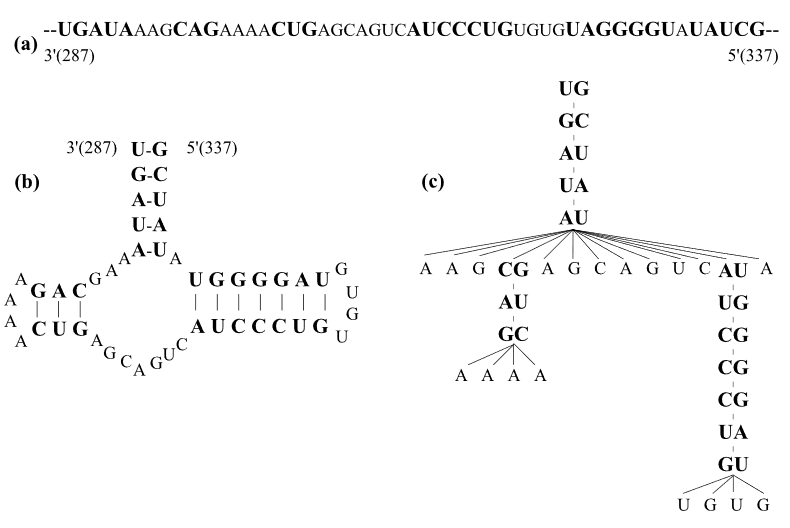
\includegraphics[width=14cm,clip]{Figures/RNATreeRepresentation}
		\label{RNA structures and forest representation} 
		\caption{RNA structures and forest representation. From ~\cite{Liang2012} (a) A segment of the RNA GI: 2347024 primary structure, (b) its secondary structure, (c) its forest representation}. 
\end{figure}

The secondary structure of RNA plays an important role in its functions preforming. In biology, it is presumed that a preserved biological function corresponds to a preserved molecular structure. Therefore, the comparison secondary structures of RNA is required in many biology problems with RNA involving, which helps reveal information regarding RNA functions.

We designed and implemented a new space and time efficient algorithm to compute the tree edit distance. Compared to other currently existing algorithm, the new algorithm use the best decomposition strategy for trees, which creates the least number of the relevant sub-problems. 

The thesis is organized as follows. Chapter 2 introduces the tree edit distance problem and the related work of tree edit distance algorithm. A number of related path decomposition algorithms are described in this chapter. A detailed explanation of the design and implementation of our improved algorithm follows in Chapter 3.Besides, another algorithmic improvement is introduced in Chapter 4. The evaluation of the new method is performed in Chapter 5 by comparing it with other leading methods and we conclude in Chapter 6.

\doublespacing
\chapter{Background}
This chapter introduces the tree editing problem and the related algorithms. The underlying concepts of the tree editing problem are first provided, followed by a naive algorithm. Then a number of improved algorithms based on closely related dynamic programming approaches are introduced. 

\section{String Edit Distance Problem}
Before we introduce the tree edit distance problem, we first describe the string edit distance problem because the string edit distance problem can be seen as a special case of the tree edit distance problem.

First introduced by Wagner and Fischer~\cite{wagner1974string}, the string edit distance problem is to find the minimum cost to change one string$S_1$ into the other$S_2$ by a sequence of edit steps. The string edit distance problem can be solved by dynamic programming. The string edit distance $d(S_1, S_2)$ can be computed by Equation 2.1  where $u$ and $v$ are both the last elements or the first element of string $S_1$ and $S_2$. The cost of the three basic edit operations( substitution, deletion and insertion) are $\delta(u, v)$, $\delta(u, \varnothing)$ and $\delta(\varnothing, v)$.

\begin{definition}
(String Edit Distance)
The edit distance between strings $S_1$ and $S_2$ is the minimum cost to change $S_1$ to $S_2$ via a sequence of basic edit steps. 
\end{definition}

\section{Tree Edit Distance Problem}

The tree edit distance problem was first introduced by Tai as a generalization of the string edit distance problem~\cite{wagner1974string}. 

\begin{definition}
(Tree Edit Distance)
The edit distance between two trees $T_1$ and $T_2$ is the minimum cost to change $T_1$ to $T_2$ via a sequence of basic edit steps. 
\end{definition}

Analogous to the string edit distance problem, the basic operations are substitution with the cost $\delta(t_1, t_2)$, insertion with the cost $\delta(\varnothing, t_2)$ and deletion with the cost $\delta(t_1, \varnothing)$, where $t_1$ and $t_2$ is a node in tree $T_1$ and $T_2$ respectively. The concept of basic operations in the tree edit distance problem is similar to that in the string edit distance problem. Substitution means changing a tree node into another. Insertion first insert a node into a tree. If the inserted node is the children of a node in the tree, the children of this node become the children of the inserted node. In contrast to insertion, deletion first delete a node from a tree then the children of the deleted node become the children of the parent of the deleted node. Figure 2.1 illustrates these editing operations.

\begin{figure}
		\centering
		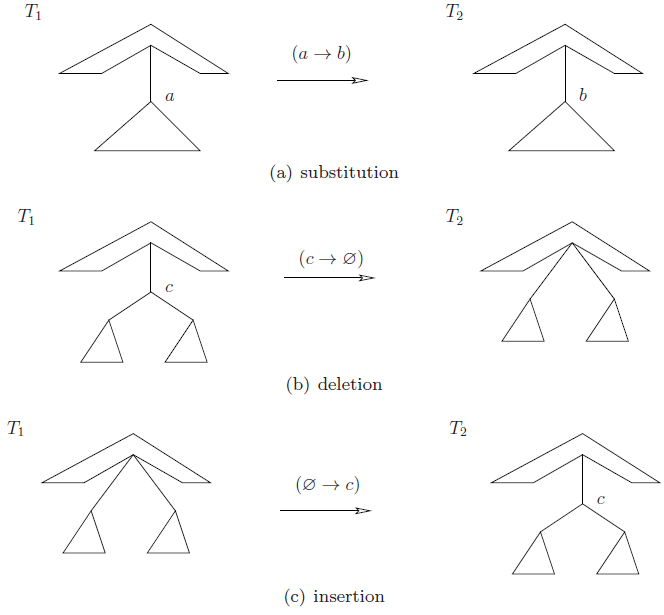
\includegraphics[width=11cm,clip]{Figures/TreeEditingOperation}
		\label{Basic tree edit operations} 
		\caption{Basic tree edit operations From ~\cite{chen2015review}. (a) substitution, (b) deletion, (c) insertion.}
\end{figure}

In this thesis, we focus on the general editing problem, which means no additional constraints are added on the order of insertions and deletions. In other words, insertions and deletions can take place in any order at any node within the tree. However, the substitution operation should satisfy the following constraints:

1. One-to-one relationship: A node in one tree can be replaced by at most one node in another tree. 

2. Sibling order is preserved: For any two substitution steps($t_1[i] \to t_2[j]$) and ($t_1[i'] \to t_2[j']$), $t_1[i]$ is to the left of $t_1[i']$ if and only if $t_2[j]$ is an ancestor of $t_2[j']$.

3. Ancestor order is preserved: For any two substitution step($t_1[i] \to t_2[j]$) and ($t_1[i'] \to t_2[j']$), $t_1[i]$ is an ancestor of $t_1[i']$ if and only if $t_2[j]$ is an ancestor of $t_2[j']$.

These constraints of the preservation of sibling and ancestor order are shown in Figure 2.2.

\begin{figure}
		\centering
		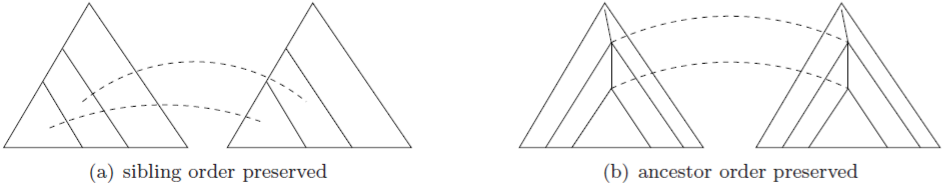
\includegraphics[width=14cm,clip]{Figures/TreeEditingOperationConstraint}
		\label{Sibling orders and ancestor orders preservation} 
		\caption{Tree editing constraints on sibling orders and ancestor orders preservation From ~\cite{chen2015review}. (a) sibling order preservation. (b) ancestor order preservation.}
\end{figure}

\section{Preliminaries}
Before we study the tree edit distance problem, it would be beneficial to define some notations, which can help analyze the algorithm clearly. 

Firstly, trees and forests should be clearly defined as they are objects in algorithms. 

\begin{definition}
(Tree and forests)
A node can be a tree. A tree is a node connected to an ordered sequence of disjoint trees. Such a sequence of tree is called a forest~\cite{dulucq2005decomposition}. 
\end{definition}

In this thesis, we only consider ordered and labeled tree. The word forest may be used for denoting forests, trees as well as a node which are reduced from a tree after a series of deletions. 

Some classical notations for trees and forests are introduced.  

\begin{notation} Let T be a tree, which is composed of a node $l$ connected to the sequence of trees $T_1, \cdots ,T_n$, T can be written as $l(T_1  \comp \cdots \comp T_n)$.
\begin{itemize}
\item $r(T)$ denotes the root of T, which is $l$ in the tree representation form of $l(T_1 \comp \cdots \comp T_n)$.
\item $T^{\comp}$ denotes the forest F after deleting r(T), that is $T_1 \comp \cdots \comp T_n$.
\item $lr(T)$ denotes the root of the leftmost tree in the forest $T^{\comp}$, that is the root of $T_1$.
\item $rr(T)$ denotes the root of the rightmost tree in the forest $T^{\comp}$, that is the root of $T_n$.
\end{itemize}
\end{notation}

\begin{notation}Let F be a forest of the form of $T_1 \comp \cdots \comp T_n$, where $T_1, \cdots ,T_n$ are trees in the forest.

\begin{itemize}
\item $\left\vert F \right\vert$ denotes the size of F, which is the number of nodes in the forest.
\item $\#leaves(F)$ denotes the number of leaves of F.
\item $depth(F)$ denotes the depth of F, that is the maximal depth of the trees in F.
\item $F(i)$, where i is a node of F, denotes the sub-tree of F rooted at i.
\item $F - i$, where i is a node of F, denotes the forest after deleting node i.
\item $lr(F)$ denotes the root of the leftmost tree in the forest $T_1 \comp \cdots \comp T_n$, that is the root of $T_1$.
\item $rr(F)$ denotes the root of the rightmost tree in the forest $T_1 \comp \cdots \comp T_n$, that is the root of $T_n$.
\end{itemize}
\end{notation}

\section{Recursive Decomposition Solution}
Before we study the recursive decomposition in the tree edit distance problem, we recall the the recursive decomposition in the string edit distance problem. The string edit distance problem can be solved by measuring the distance for all pairs of prefixes or suffixes of two strings.

The edit distance between two strings $S_1$ and $S_2$ can be computed by the following equation:
\begin{align}
d(S_1, S_2) = min \begin{cases}
	  	d(S_1 - u , S_2) + \delta(u, \varnothing) \\ 
      	d(S_1, S_2 - v) + \delta(\varnothing, v) \\ 
    	d(S_1 - u, S_2 - v) + \delta(u, v) & \\ 
    \end{cases}
\end{align}

It is a right decomposition if and only if $u$ and $v$ are both the last element of the string $S_1$ and $S_2$. Similarly, when $u$ and $v$ are both the first element of the string $S_1$ and $S_2$, it is a left decomposition. Implementation of the string edit distance is the completion with a two-dimensional table, which gives a $\mathcal{O}(n^2)$ solution.

Analogous to the string edit distance problem, the tree edit distance can be solved in a recursive decomposition way. To compute the tree edit distance,  the roots of the trees are the first elements to decompose. The Equation 2.2 computes the tree-to-tree distance.

Let $T_1$ and $T_2$ be two trees, 
\begin{align}
d(T_1, T_2) = min \begin{cases}
	  	d(T_1 - r(T_1) , T_2) + \delta(r(T_1), \varnothing) \\ 
      	d(T_1, T_2 - r(T_2)) + \delta(\varnothing, r(T_2)) \\ 
    	d(T_1 - r(T_1), T_2 - r(T_2)) + \delta(r(T_1), r(T_2)) & \\
    \end{cases}
\end{align}

The decomposition to trees create sub-problems for forests($T_1 - r(T_1), T_2 - r(T_2)$). Similar to the Equation 2.1 for the calculation of the string edit distance, let $F_1$ and $F_2$ be two forests and $u$ and $v$ be two nodes in forest $F_1$ and $F_2$ respectively, the forest-to-forest distance can be computed by equation as follows: 
\begin{align}
d(F_1, F_2) = min \begin{cases}
	  	d(F_1 - u , F_2) + \delta(u, \varnothing) \\ 
      	d(F_1, F_2 - v) + \delta(\varnothing, v) \\ 
    	d(F_1 - F(u), F_2 - F(v)) + \delta(F(u), F(v))& \\ 
    \end{cases}
\end{align}

Analogous to the string edit distance problem, the computation of forest-to-forest takes on two possible directions: left and right decomposition. Figure 2.3 illustrates the left and right decomposition.
\begin{itemize}
\item left decomposition where $u$ and $v$ are $lr(F_1)$ and $lr(F_2)$ respectively.(Figure 2.3 (a-1), (b-1), (c-1)).
\item right decomposition where $u$ and $v$ are $rr(F_1)$ and $rr(F_2)$ respectively.(Figure 2.3 (a-2), (b-2), (c-2)).
\end{itemize}

\begin{figure}
		\centering
		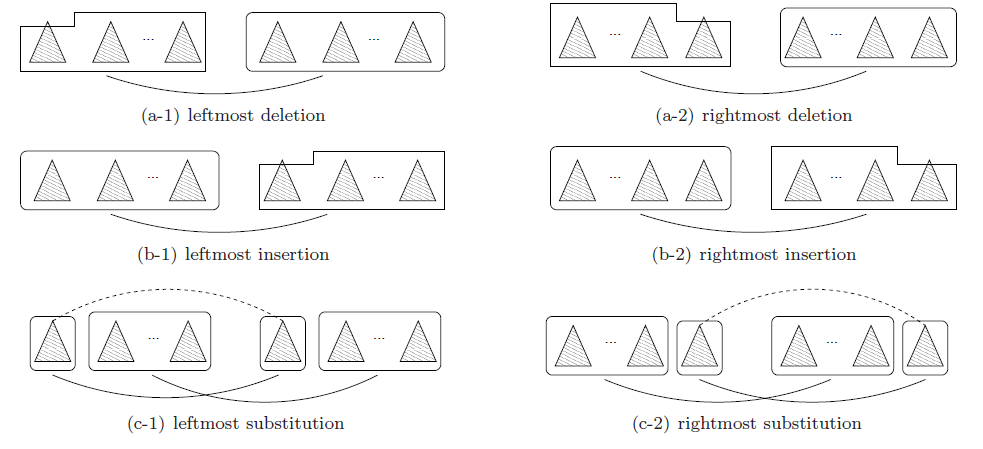
\includegraphics[width=16cm,clip]{Figures/LeftRightDecomposition}
		\label{Left and Right Recursive composition} 
		\caption{Left and Right decomposition From ~\cite{Chen2014}. (a-1) leftmost deletion. (b-1) rightmost insertion. (c-1) leftmost substitution. (a-2) rightmost deletion. (b-2) rightmost insertion. (c-2) rightmost substitution.}
\end{figure}

\section{Relevant SubForests and SubTrees}
The recursive decomposition creates relevant sub-forests recursively. 

\begin{definition}
(Relevant sub-forest)
The relevant sub-forests are the forests that appear in the recursive calls in the Equation 2.2 and 2.3. 
\end{definition}

The set of all sub-forest resulting from any decomposition from the forest F is called the full decomposition, denoted by $\mathcal{A}(F)$.

\begin{definition}
(Full decomposition)
The full decomposition of a tree is the set of all sub-forests of F obtained by recursively removing the leftmost and rightmost root nodes, $lr(F)$ and $rr(F)$, from F and the resulting sub-forests. 
\begin{equation*}
\mathcal{A}(\varnothing) = \varnothing
\end{equation*}
\begin{equation*}
\mathcal{A}(F) = \{F\} \cup \mathcal{A}(F - rr(F)) \cup \mathcal{A}(F - lr(F))
\end{equation*}
\end{definition}

Figure 2.4 illustrates the relevant sub-forests of a tree resulting from the full decomposition of a tree F.
\begin{figure}
		\centering
		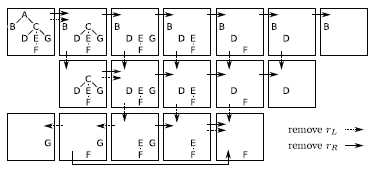
\includegraphics[width=8cm,clip]{Figures/FullDecomposition}
		\label{Relevant Sub-forests Resulting From the Full Decomposition} 
		\caption{Relevant sub-forests resulting from the full decomposition. From ~\cite{pawlik2015efficient}.}
\end{figure}

To decompose a tree, leftmost or rightmost root node can be chosen at each recursive step, resulting in the path decomposition, which is a subset of the full decomposition. Each choice of direction in each step is called a decomposition strategy. The set of decomposition strategies can be indicated by a root-leaf path.

\begin{definition}
(Root-leaf path)
The root-leaf path indicates the choice of decomposition strategy at each step in the recursive call. If the rightmost root of forest $F_1$ or $F_2$ is on the path, then $u = lr(F_1)$ and $v = lr(F_2)$ in the Equation 2.3. On the contrary, if the leftmost root of forest $F_1$ or $F_2$ is on the path, then $u = rr(F_1)$ and $v = rr(F_2)$
\end{definition}

The set of sub-forests decomposed by a root-leaf path from the forest F is called the path decomposition, denoted by $\mathcal(F)(F)$.

\begin{definition}
(Path decomposition) Path decomposition is a set of sub-forests of F obtained by recursively removing the leftmost or rightmost root nodes, $lr(F)$ and $rr(F)$, from F and the resulting sub-forests. 
\begin{equation*}
\mathcal{F}(\varnothing) = \varnothing
\end{equation*}
\begin{equation*}
\mathcal{F}(F) = \{F\} \cup \begin{cases}
	  	\mathcal{F}(F - rr(F))\\ 
      	\mathcal{F}(F - lr(F))\\ 
    \end{cases}
\end{equation*}
\end{definition}




Figure 2.5(a) is an example of relevant sub-forests that result from the leftmost path decomposition, which successively delete the rightmost root of the resulting forest. This creates 15 relevant sub-forests.Symmetrically, the rightmost path decomposition creates 11 relevant sub-forests(Figure 2.5(b)).

\begin{figure}
		\centering
		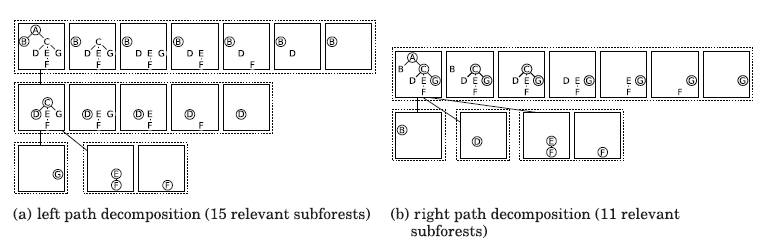
\includegraphics[width=16cm,clip]{Figures/PathDecomposition}
		\label{Relevant Sub-trees from the leftmost path decomposition and the rightmost path decomposition} 
		\caption{Relevant sub-forests. From ~\cite{pawlik2015efficient}. (a) Relevant sub-forests from the leftmost path decomposition. (b) Relevant sub-forests from the rightmost path decomposition.}
\end{figure}

\begin{definition}
(Relevant sub-trees)
The relevant sub-trees of tree T for a root-leaf path are all sub-trees that result from removing the path from T, that is, all sub-trees of T that are connected to a node of the path.  
\end{definition}

As shown in Figure 2.6, the black nodes belong to the root-leaf path and the white nodes are connected to one of the node on the path. The sub-trees rooted at the white nodes are sub-tree result from the path decomposition. 

\begin{figure}
		\centering
		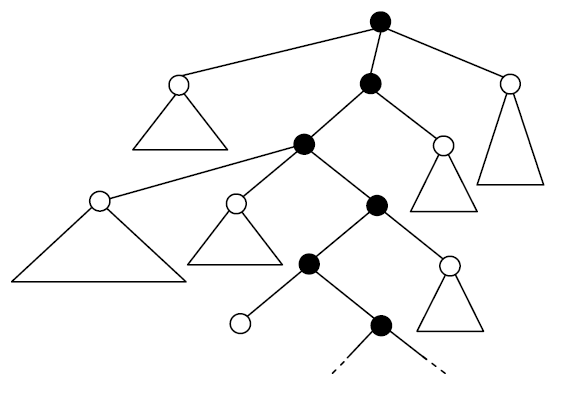
\includegraphics[width=8cm,clip]{Figures/RelevantSubtrees}
		\label{Relevant Sub-trees from the path decomposition} 
		\caption{Relevant sub-forests. From ~\cite{demaine2009optimal}.}
\end{figure}

\begin{notation}
Let T be a tree, $\gamma$ be a root-leaf path.
\begin{itemize}
\item $\Gamma(T)$ denotes the set of roots of relevant sub-trees partitioned by the path $\gamma$.
\end{itemize}

\end{notation}

So far, we have considered relevant sub-trees and sub-forests with respect to a single root-leaf path. If a root-leaf path can be defined for each of the resulting sub-trees of tree T,  the path decomposition can be recursively applied to all resulting sub-trees. This procedure is called the recursive path decomposition.
\section{Bottom-up Enumeration}
The space-efficient implementations of the tree edit distance use a bottom-up approach, which computes distance between smaller pairs of sub-trees first. In contrast to the top-down decomposition, the bottom-up enumeration order the sub-trees computation carefully to make sure all the sub problems from the Equation 2.2 and 2.3 have already been computed beforehand. 

The order of bottom-up enumeration is closely related to the top-down recursive decomposition. The top-down recursive path decomposition can be categorized into two approaches.

\begin{itemize}
\item the recursion direction is fixed to be either leftmost or rightmost,
\item the recursion direction may vary between leftmost and rightmost.
\end{itemize}

For either approach, we need an approach to enumerate the sub-problems. For the fixed direction recursion, one way to enumerate the sub problems is enumerate sub-trees as well as the sub-forests contained in each sub-tree in left-to-right or right-to-left postorder. 

\begin{itemize}
\item LR-postorder: The sub-trees as well as the sub-forests contained in each sub-trees are enumerated in left-to-right postorder.
\item RL-postorder: The sub-trees as well as the sub-forests contained in each sub-trees are enumerated in right-to-left postorder.
\end{itemize}

Figure 2.7 is an example of relevant sub-forests that result from tree T and each of its relevant sub-trees with respect to the leftmost path. The top-down view gives the recursive right decomposition while the bottom-up gives the left-to-right postorder enumeration. 

\begin{figure}
		\centering
		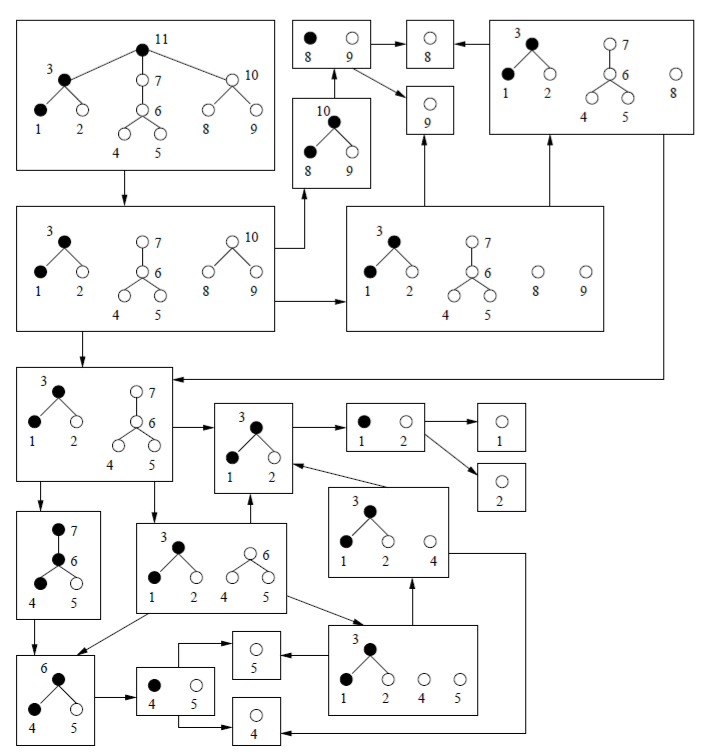
\includegraphics[width=12cm,clip]{Figures/LeftToRightEnumeration}
		\label{Relevant Sub-forests that Result From the Leftmost Path Decomposition} 
		\caption{Relevant sub-forests that result from the leftmost path decomposition. From ~\cite{Chen2014}.}
\end{figure}

To enumerate the full decomposition, two approaches can be used, which is suffix-prefix and prefix-suffix postorder enumeration. In prefix-suffix postorder enumeration leftmost root is fixed then enumerate each nodes in the sub-tree, whereas rightmost root is fixed then enumerate each nodes in the sub-tree in suffix-prefix postorder. 

\begin{itemize}
\item prefix-suffix postorder: Enumerate the rightmost root in left-to-right postorder then enumerate the leftmost root in the tree. 
\item suffix-prefix postorder: Enumerate the leftmost root in right-to-left postorder then enumerate the rightmost root in the tree.
\end{itemize}

Figure 2.8 and Figure 2.9 is the example of prefix-suffix order enumeration and suffix-prefix order enumeration respectively. In Figure 2.10, sub-forests having the same rightmost root are in contiguous boxes while sub-forests having the same leftmost root are in contiguous boxes.

\begin{figure}
		\centering
		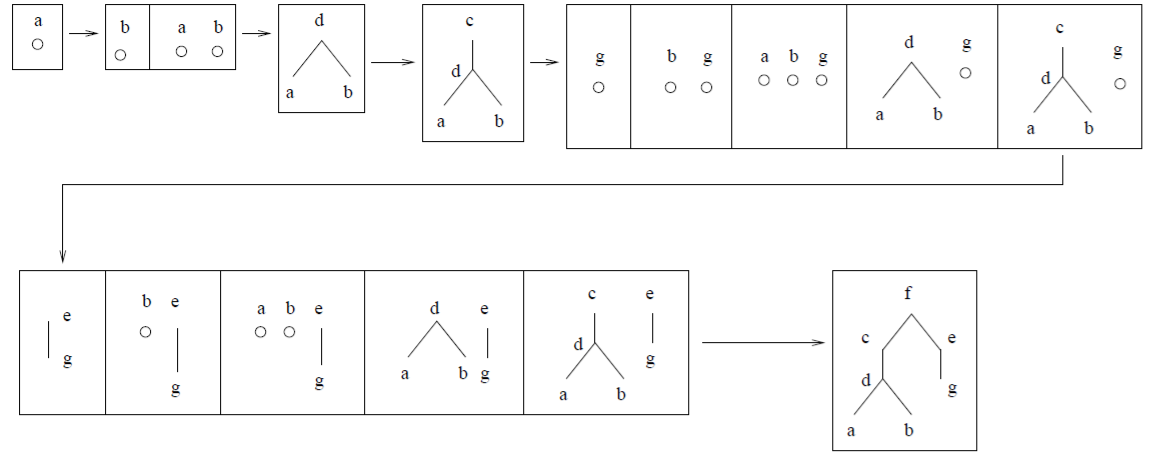
\includegraphics[width=12cm,clip]{Figures/PrefixSuffixPostorder}
		\label{Prefix-suffix Postorder Enumeration} 
		\caption{An example of enumerating subforests in prefix-suffix postorder. From ~\cite{Chen2014}.}
\end{figure}

\begin{figure}
		\centering
		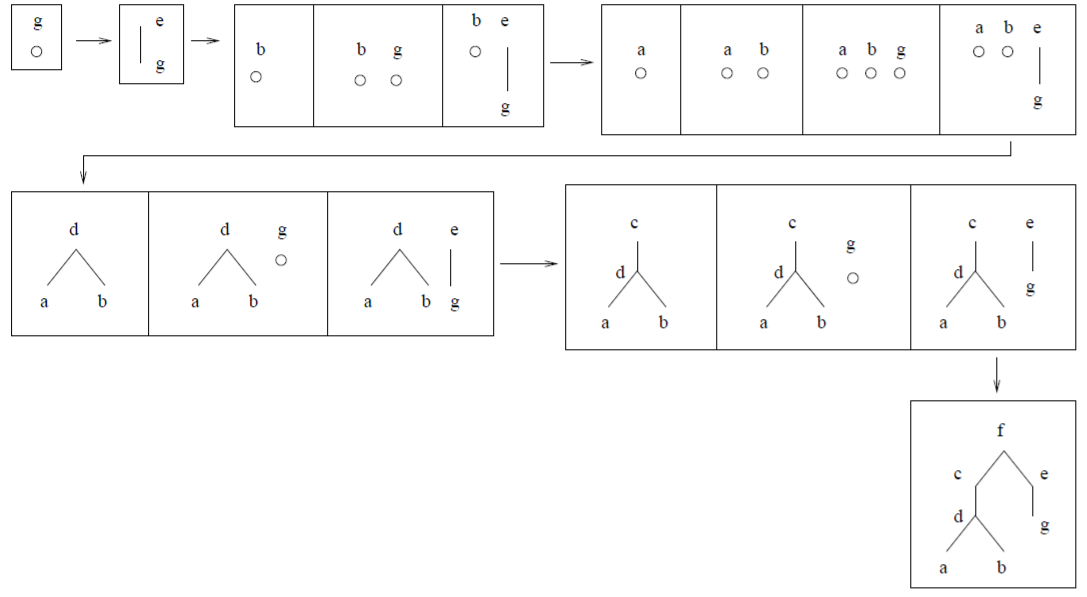
\includegraphics[width=12cm,clip]{Figures/SuffixPrefixPostorder}
		\label{Suffix-prefix Postorder Enumeration} 
		\caption{An example of enumerating subforests in suffix-prefix postorder. From ~\cite{Chen2014}.}
\end{figure}

\section{A Simple Algorithm}
In this section, we provide a simple algorithm to compute the tree edit distance, which runs in $\mathcal{O}(m^{2}n^{2})$, where $m$ and $n$ are the size of tree. To compute the tree edit distance between two pairs, we need to calculate the distance of all sub-forests pairs, which are enumerate in prefix-suffix or suffix-prefix postorder. 

\begin{lemma} The full decomposition takes $\mathcal{O}(\left\vert T \right\vert ^ {2})$ steps, where $\left\vert T \right\vert$ is the size of the tree.
\end{lemma} 
\begin{proof}
We consider the prefix-suffix postorder only as the suffix-prefix postorder is symmetrical. 
Let $f_{i}$ be the number of sub-forests with distinct leftmost roots which contain $t_i$ as the rightmost root. As menetioned in section 2.6, to enumerate the full decomposition in prefix-suffix postorder, first fix the rightmost root then enumerate the leftmost root in the tree in right-to-left postorder. Summing over all nodes to enumerate, we have $\sum_{i=1}^{\left\vert T \right\vert} \leq \sum_{i=1}^{\left\vert T \right\vert} \left\vert T \right\vert = \mathcal{O}(\left\vert T \right\vert^{2})$
\end{proof}

By enumerating all pairs of sub-forests between two trees, the tree edit distance can be calculated.  Here is a simple algorithm runs in $\mathcal{O}(m^2n^2)$ time using $\mathcal{O}(m^2n^2)$ space.

\IncMargin{1em}
\begin{algorithm}
  \caption{Compute tree edit distance by enumerating all pairs in $\mathcal{O}(m^2n^2)$ time.}
  \SetKwInOut{Input}{inputs}
  \SetKwInOut{Output}{output}
  \SetKwData{TreeA}{$T_1$}
  \SetKwData{TreeB}{$T_2$}
  \SetKwData{SizeOfTreeA}{$\left\vert T_1 \right\vert$}
  \SetKwData{SizeOfTreeB}{$\left\vert T_2 \right\vert$}
  \SetKwFunction{POSTORDER}{POSTORDER}{}{}

  \Input{ (\TreeA , \TreeB), with \SizeOfTreeA = $m$ and \SizeOfTreeB = $n$ }
  \Output{$d(T_1[i], T_2[j])$ for $1 \leq i \leq m$ and $1 \leq j \leq n$}
    $L_1 \gets \POSTORDER(T_1)$\;
    $L_2 \gets \POSTORDER(T_2)$\;
    \For{$i=1$ \KwTo $\left\vert L_1 \right\vert$} {
		\For{$j=1$ \KwTo $\left\vert L_2 \right\vert$} {
			compute $d(L_1[i], L_2[j])$ as in Equation 2.3
		}    
    }
    $d(T_1[i], T_2[j]) \gets d(L_1[\left\vert L_1 \right\vert][\left\vert L_2 \right\vert])$\;
    \KwRet{$d(T_1[i], T_2[j])$}\;
\end{algorithm}
\DecMargin{1em}

\begin{lemma}
The upper bound of the post-order enumeration method for tree edit distance problem is $\mathcal{O}(m^2n^2)$, where $m$ and $n$ are the size of two trees.
\end{lemma}
\begin{proof}
From lemma 2.7.1, the upper bound(full decomposition with no assumption on the strategy) of the number of relevant sub-forests for one tree of size $n$ is $\mathcal{O}(n^2)$. Therefore, the upper bound of the relevant sub-forests pairs of trees of sizes $m$ and $n$ respectively is $\mathcal{O}(m^2n^2)$. This concludes the proof.
\end{proof}

\section{Improved Algorithmic Path Strategies}
Leftmost or rightmost root node is chosen at each recursive step, resulting in the path decomposition, which is the subset of the full decomposition. We use a root-leaf path to indicate the set of decomposition strategies.

Different path decomposition creates different number of relevant sub-forests. Figure 2.10 and Figure 2.11 is an example of different sub-forests that result from different path decomposition strategies. In Figure 2.10, the path is rightmost path, and in Figure 2.11, the path is leftmost path. This gives respectively 7 and 9 sub-forests. Therefore, to make further improvement we look for ways to take advantage of the overlap among sub-forests that are contained in the same sub-tree, and the overlap of sub-trees as well. 

\begin{figure}
		\centering
		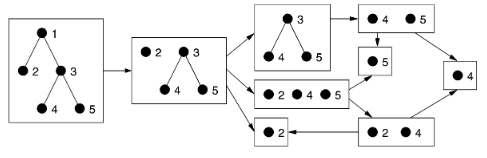
\includegraphics[width=12cm,clip]{Figures/LeftmostPathDecomposition}
		\label{Relevant Sub-forests that Result From the Leftmost Path Decomposition} 
		\caption{Relevant sub-forests that result from the leftmost path decomposition. From ~\cite{dulucq2005decomposition}.}
\end{figure}

\begin{figure}
		\centering
		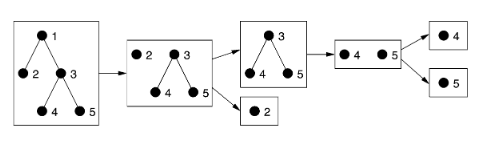
\includegraphics[width=12cm,clip]{Figures/RightmostPathDecomposition}
		\label{Relevant Sub-forests that Result From the Rightmost Path Decomposition} 
		\caption{Relevant sub-forests that result from the rightmost path decomposition. From ~\cite{dulucq2005decomposition}.}
\end{figure}

The current state-of-the art path strategies are leftmost(rightmost) paths on both tree, heavy paths on one tree as well as heavy paths on both trees.

\section{Zhang and Shasha's Algorithm}

Zhang and Shasha's algorithm~\cite{zhang1989simple} fixes the direction in each recursion, say right decomposition. The situation for the recursive left decomposition is symmetrical to that for the recursive right decomposition. 

\begin{figure}
		\centering
		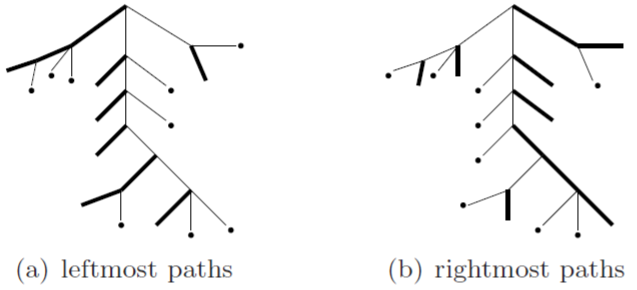
\includegraphics[width=12cm,clip]{Figures/LeftmostPathandRightmostPath}
		\label{Leftmost Paths and Rightmost Paths} 
		\caption{Leftmost paths and rightmost paths in a tree and its resulting sub-trees From ~\cite{Chen2014}.}
\end{figure}

Full decomposition is not needed in the Zhang and Shasha's algorithm since the direction to decompose is fixed. This means that only the path decomposition to the whole tree and its resulting sub-trees is needed instead of the full decomposition. This means that the enumeration of the Zhang and Shasha's algorithm will be in LR-postorder while the symmetrical rightmost paths algorithm used RL-postorder enumeration. See Figure 2.12(a) as an example of the leftmost paths applied the whole tree and its resulting sub-trees and Figure 2.12(b) is the example of rightmost paths.

Taking the advantage of the overlap among sub-trees, all sub-trees sharing the same leftmost leaf can be handled together. In other words, a set of sub-tress along the leftmost path can be handled together with the LR-postorder enumeration to avoid redundant computation.

The root of each relevant sub-trees resulted from the leftmost paths is refereed to as an "LR-keyroot", which is defined as follows.

\begin{definition}
(LR-keyroots). An LR-keyroot is either the root of T or has a left sibling.
\end{definition}

The procedure of the Zhang and Shasha's algorithm as follows. First we identify all LR-keyroots and sort them in LR-postorder. Then enumerate each pairs of relevant sub-trees in order and calculate the distance between them. 

\IncMargin{1em}
\begin{algorithm}
  \caption{Zhang and Shasha's Algorithm}
  \SetKwInOut{Input}{inputs}
  \SetKwInOut{Output}{output}
  \SetKwData{TreeA}{$T_1$}
  \SetKwData{TreeB}{$T_2$}
  \SetKwData{SizeOfTreeA}{$\left\vert T_1 \right\vert$}
  \SetKwData{SizeOfTreeB}{$\left\vert T_2 \right\vert$}
  \SetKwFunction{POSTORDER}{LR\_KEYROOT\_POSTORDER}{}{}
  \SetKwFunction{TREEDISTANCE}{TREE\_TREE\_DISTANCE}{}{}

  \Input{ (\TreeA , \TreeB), with \SizeOfTreeA = $m$ and \SizeOfTreeB = $n$ }
  \Output{$d(T_1[i], T_2[j])$ for $1 \leq i \leq m$ and $1 \leq j \leq n$}
    $L_1 \gets \POSTORDER(T_1)$\;
    $L_2 \gets \POSTORDER(T_2)$\;
    \For{$i=1$ \KwTo $\left\vert L_1 \right\vert$} {
		\For{$j=1$ \KwTo $\left\vert L_2 \right\vert$} {
			$\TREEDISTANCE(T_1(L_1[i]), T_2(L_2[j]))$
		}    
    }
    $d(T_1[i], T_2[j]) \gets d(L_1[\left\vert L_1 \right\vert][\left\vert L_2 \right\vert])$\;
    \KwRet{$d(T_1[i], T_2[j])$}\;
\end{algorithm}
\DecMargin{1em}

In function TREE\_TREE\_DISTANCE in Algorithm 2, the leftmost root is fixed and the rightmost roots are enumerated to construct relevant sub-forests. The enumeration algorithm is shown in algorithm 3.

\IncMargin{1em}
\begin{algorithm}
  \caption{TREE\_TREE\_DISTANCE}
  \SetKwInOut{Input}{inputs}
  \SetKwInOut{Output}{output}
  \SetKwData{TreeA}{$T_1(a)$}
  \SetKwData{TreeB}{$T_2(b)$}
  \SetKwData{RA}{$a$}
  \SetKwData{RB}{$b$}
  \SetKwFunction{POSTORDER}{LR\_POSTORDER}{}{}

  \Input{ (\TreeA , \TreeB)}
  \Output{$d(T_1(a), T_2(b))$}
    $L_1 \gets \POSTORDER(T_1(a))$\;
    $L_2 \gets \POSTORDER(T_2(b))$\;
    \For{$i=1$ \KwTo $\left\vert L_1 \right\vert$} {
		\For{$j=1$ \KwTo $\left\vert L_2 \right\vert$} {
			$rr\_F_1 \gets L_1[i]$\;
			$rr\_F_2 \gets L_2[j]$\;
			
			\uIf{$rr\_F_1 == lr(T_1(a)) \land rr\_F_2 == lr(T_2(b))$ } {
				compute $d(T_1(rr\_F_1),  T_2(rr\_F_2))$ as in Equation 2.2\;
			}
			\uElse {
				compute $d((lr(T_1(a), rr\_F_1), (lr(T_2(b)), rr\_F_2))$ as in Equation 2.3\;		
			}		
		}    
    }
    \KwRet{$d(T_1(a), T_2(b))$}\;
\end{algorithm}
\DecMargin{1em} 

\begin{lemma}
The time complexity of Zhang and Shasha's algorithm is $\mathcal{O}(mn \times min\{depth(T_1), \#leaves(T_1)\} \times min\{depth(T_2), \#leaves(T_2)\})$
\end{lemma}
\begin{proof}
Each sub problems can be solved in constant time. Thus, the time complexity can be counted by the number of sub problems. According to the enumeration scheme from algorithm 3, the number can be counted by the occurring of each node representing as the rightmost root in relevant sub-forests. The maximal times a node representing the rightmost root of relevant sub-forests can be estimated by the maximal number of non-leaf LR-keyroots that a path in the tree may contain. Firstly, since the number of LR-keyroots on any path is bounded by the depth of the path, the number of sub problems is bounded by $\#depth(T)$. Secondly, the number of sub-trees can not exceed the number of leaves as each relevant sub-trees in the Zhang and Shasha's algorithm have distinct leftmost leaves. Therefore, the number of relevant sub-trees decomposed by a leftmost path is bounded by $depth(T)$ or $\#leaves(T)$, whichever is smaller. Therefore the number of sub-forests in either tree is $\left\vert T \right\vert \times min\{depth(T), \#leaves(T)\}$  
\end{proof}
\begin{lemma}
The tree edit distance problem can be solved in $\mathcal{O}(mn)$ space, where $m=\left\vert T_1 \right\vert$ and $n=\left\vert T_2 \right\vert$
\end{lemma}
\begin{proof}
Dynamic programming method is used to implement, which fills out two $m \times n$ tables. One permanent matrix stores the tree-tree distance and the other temporary matrix stores the forest-forest distance. The temporary forest-forest distance matrix can be overwritten when the computation moves from one pair of relevant sub-trees to another pair. Besides, the permanent tree-tree distance matrix are fetched for use in computing forest-forest distances.
\end{proof}
\section{Klein's Algorithm}
Zhang and Shasha's algorithm improves the time complexity by taking the advantage of the overlap of  sub-forests with the same leftmost root. However, the running time can be improved in some trees as it is dependent on shapes of trees. Kelvin~\cite{klein1998computing} explored and designed a new decomposition strategy based on a type of path called "heavy path". Zhang and Shasha's algorithm ignores shapes of trees and fixes the direction in each decomposition steps while the direction may change in each steps according to different tree shapes. 

Heavy child and heavy paths was first introduced by Harel and Tarjan\cite{harel1984fast}. The definition is as follows.

\begin{definition}
(Heavy Child)
For any node t in Tree T, the heavy child is the root of the largest sub-trees among the sibling sub-trees, denoted by $heavy(t)$.
\end{definition}

\begin{definition}
(Heavy Path)
The descending path of Tree T from root to leaf consists of the sequence of nodes $r, heavy(r), heavy(heavy(r)) \cdots$ is called the heavy path, denoted by $P(T)$
\end{definition}

Figure 2.13 is an example of heavy paths. In the left picture, a tree's heavy path is indicated in bold. The figure on the right depicts heavy paths applied to the whole tree and its relevant sub-trees.

\begin{figure}
		\centering
		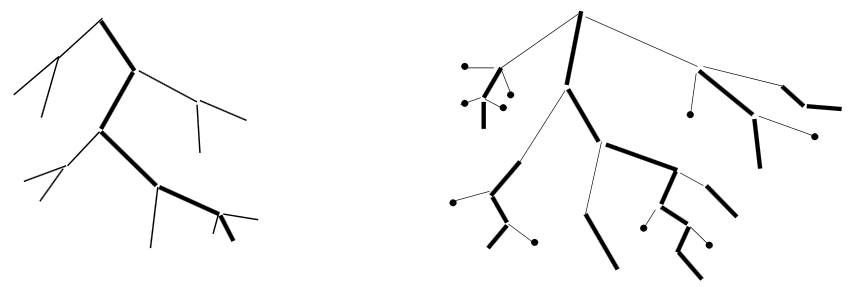
\includegraphics[width=12cm,clip]{Figures/HeavyPaths}
		\label{Heavy Paths} 
		\caption{Heavy Paths to a tree and its relevant sub-trees From ~\cite{klein1998computing}.}
\end{figure}

Let $F$ be a forest denoted as $l(f) \comp t$, where $l(f)$ is the leftmost tree in the forest, $t$ be the rest of the forest and $F'$ be another forest to compare. In Klein's algorithm, the procedure of the decomposition using the heavy path of the tree is as follows:

\begin{enumerate}
\item if $l$ belongs to the heavy path, apply right decomposition, otherwise apply left decomposition
\item apply this scheme recursively to all relevant sub-forests of $l(f) \comp t$
\end{enumerate}

Figure 2.14 illustrates the this procedure. For each step, the nodes on the heavy path are indicated by circles. 

\begin{figure}
		\centering
		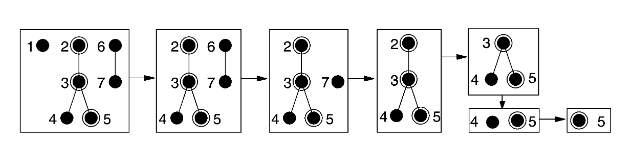
\includegraphics[width=12cm,clip]{Figures/KleinAlgorithmExample}
		\label{Example of Decomposition for Klein's Algorithm} 
		\caption{Example of decomposition for Klein's algorithm From ~\cite{klein1998computing}.}
\end{figure}

Symmetrical to Klein's decomposition, right decomposition can be first applied to relevant sub-forests then left decomposition. Let $F$ be a forest denoted as $l(f) \comp t$, where $l(f)$ is the leftmost tree in the forest, $t$ be the rest of the forest and $F'$ be another forest to compare, the procedure is shown as follows:

\begin{enumerate}
\item if $l$ belongs to the heavy path, apply left decomposition, otherwise apply right decomposition
\item apply this scheme recursively to all relevant sub-forests of $l(f) \comp t$
\end{enumerate} 

Two ways of top-down decomposition give two ways of bottom-up enumeration, referred as  "H-postorder". Nodes on the right side of the heavy child can first be enumerated in left-to-right postorder then nodes on the left side are enumerated in right-to-left postorder. Alternatively, the second version is symmetrical to the first one, i.e., right-to-left postorder then left-to-right postorder intermittently. Figure 2.15 is an example of H-postorder enumeration in Klein's algorithm.

\begin{figure}
		\centering
		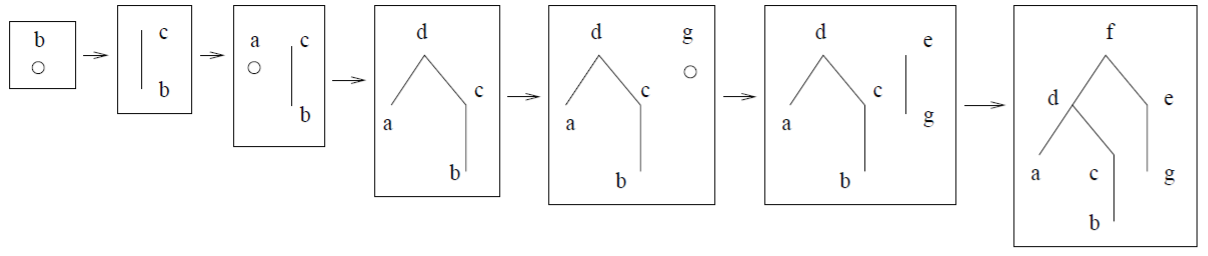
\includegraphics[width=12cm,clip]{Figures/HPostoderEnumeration}
		\label{Example of Enumerating Sub-forests in H-postorder} 
		\caption{Example of enumerating sub-forests in H-postorder From ~\cite{chen2015review}.}
\end{figure}

As listed in Algorithm 4, the keyroots in the larger tree are sorted in H-postorder. On the other hand, the full decomposition of the smaller tree is sorted in prefix-suffix or suffix-prefix postorder. Then compute each relevant sub-trees of the larger tree with respect to each relevant sub-forests of the smaller tree. 

\IncMargin{1em}
\begin{algorithm}
  \caption{Klein's Algorithm}
  \SetKwInOut{Input}{inputs}
  \SetKwInOut{Output}{output}
  \SetKwData{TreeA}{$T_1$}
  \SetKwData{TreeB}{$T_2$}
  \SetKwData{SizeOfTreeA}{$\left\vert T_1 \right\vert$}
  \SetKwData{SizeOfTreeB}{$\left\vert T_2 \right\vert$}
  \SetKwFunction{HPOSTORDER}{H\_KEYROOT\_POSTORDER}{}{}
  \SetKwFunction{FPOSTORDER}{PREFIX\_SUFFIX\_POSTORDER}{}{}
  \SetKwFunction{TREEDISTANCE}{TREE\_TREE\_DISTANCE}{}{}

  \Input{ (\TreeA , \TreeB), with \SizeOfTreeA = $m$, \SizeOfTreeB = $n$ and $m \leq n$}
  \Output{$d(T_1[i], T_2[j])$ for $1 \leq i \leq m$ and $1 \leq j \leq n$}
    $L_1 \gets \FPOSTORDER(T_1)$\;
    $L_2 \gets \HPOSTORDER(T_2)$\;
    \For{$i=1$ \KwTo $\left\vert L_1 \right\vert$} {
		\For{$j=1$ \KwTo $\left\vert L_2 \right\vert$} {
			compute $d(L_1[i], L_2[j])$ as in Equation 2.3
		}    
    }
    $d(T_1[i], T_2[j]) \gets d(L_1[\left\vert L_1 \right\vert][\left\vert L_2 \right\vert])$\;
    \KwRet{$d(T_1[i], T_2[j])$}\;
\end{algorithm}
\DecMargin{1em}
\begin{lemma}
Let $h_1, h_2, \cdots h_k$ be any nodes on the same heavy path he same path where $h_i$ is an ancestor of $h_j$ if $i < j$. Then, $\left\vert T(h_j) \right\vert \leq \left\vert T(h_i) \right\vert / 2$ if $j=i+1$
\end{lemma}
\begin{proof}
By definition, heavy child is the root of the largest sub-trees among the sibling sub-trees. Then, $\left\vert T(h_j) \right\vert \leq \left\vert T(h_i) \right\vert / 2$ is always true. Otherwise, it is a contradiction to the fact that $h_j$ is a heavy child.
\end{proof}

\begin{lemma}
The time complexity of Klein's algorithm is $\mathcal{O}(m^2n \log n)$, where $\left\vert T_1 \right\vert = m$, $\left\vert T_2 \right\vert = n$ and $m \leq n$.
\end{lemma}
\begin{proof}
Each sub problems can be solved in constant time. Thus, the time complexity can be counted by the number of sub problems. According to the enumeration scheme from algorithm 3, the number can be counted by the occurring of each node representing as the rightmost root in relevant sub-forests. The maximal times a node representing the rightmost root of relevant sub-forests can be estimated by the maximal number of non-leaf keyroots that a path in the tree may contain. From Lemma 2.10.1, for each nodes in the heavy path that is being visited, the corresponding subtree size is reduced by at least a factor of 2 with respect to its parent. In other word, it takes at most $log_2(\left\vert T \right\vert)$ steps from the root to path. That is to say, the number of sub-forests of the larger tree is bounded by $n \times log n$

Since the direction in each steps is not fixed, the full decomposition rather than the path decomposition of the smaller is needed to be considered, which creates at most $m^2$ relevant sub-forests.

To sum up, the number of pair of relevant sub-forests is $m^2n \log n$, which concludes the proof.
\end{proof}
\begin{lemma}
The space complexity of Klein's algorithm is $\mathcal{O}(mn)$, where $\left\vert T_1 \right\vert = m$, $\left\vert T_2 \right\vert = n$ and $m \leq n$. 
\end{lemma}
\begin{proof}
We use one temporary matrix of the size $m \times n$ and one permanent matrix of the size $m^2$ to store the intermediate result. The permanent matrix stores the tree-tree distance and the temporary one stores the distance between between a specific sub-tree in the larger tree and each relevant sub-forests in the full decomposition of the smaller tree. The temporary matrix can be rewritten when a new sub-tree is enumerated. Additionally, the results in the permanent tree-tree distance matrix are fetched for use in computing forest-forest distances.
\end{proof}

\section{Demaine's Algorithm}
Klein algorithm reduces the upper bound on the number of relevant sub-forests required from $\mathcal{O}(min\{depth(T), \#leaves(T)\})$ to $\mathcal{O}(\log \left\vert T \right\vert)$ for one tree. However, the cost to this strategy is having to consider all sub-forests(full decomposition) not partial sub-forests(path decomposition) in the other tree. Demaine~\cite{demaine2009optimal} improved this strategy by a way that applies the heavy path decomposition on both trees. 

Let $T_1$ and $T_2$ be two trees, assuming that $\left\vert T_1 \right\vert \leq \left\vert T_2 \right\vert$, Demaine's algorithm works as follows:

\begin{enumerate}
\item If $\left\vert T_1 \right\vert > \left\vert T_2 \right\vert$, compute $d(T_2, T_1)$
\item Recursively, compute $d(T_1, T_2(k))$ with k being the root of relevant sub-trees.
\item Compute $d(T_1, T_2)$ by enumerating full decomposition of $T_1$ in prefix-suffix or suffix-prefix postorder, and path decomposition of $T_2$ in H-postorder.
\end{enumerate}
\begin{lemma}
Let $T_1$ and $T_2$ be two trees, $R(T_1, T_2)$ be the number of relevant sub-forests pairs encountered by the algorithm, we have
\begin{equation*}
R(T_1, T_2) \leq 4(\left\vert T_1 \right\vert \left\vert T_2 \right\vert)^{\frac{3}{2}}
\end{equation*}
\end{lemma}
\begin{proof}
This can be proved by induction on $\left\vert T_1 \right\vert + \left\vert T_2 \right\vert$.

Basis: if $\left\vert T_1 \right\vert + \left\vert T_2 \right\vert = 0$, then both trees are empty and $R(T_1, T_2) = 0$ always holds.

Induction: if $\left\vert T_1 \right\vert + \left\vert T_2 \right\vert > 0$, for the case $\left\vert T_1 \right\vert \geq \left\vert T_2 \right\vert$, we have established
\begin{equation*}
R(T_1, T_2) \leq \left\vert T_2 \right\vert^2\left\vert T_1 \right\vert + \sum_{v \in \Gamma(T_1)}R(T_1(v), T_2)
\end{equation*} 
We consider the first case only for the other case when $\left\vert T_1 \right\vert < \left\vert T_2 \right\vert$ is symmetric.
Hence, by the induction hypothesis,
\begin{align}
R(T_1, T_2) &\leq \left\vert T_2 \right\vert^2\left\vert T_1 \right\vert + \sum_{v \in \Gamma(T_1)}4(\left\vert T_1(v) \right\vert \left\vert T_2 \right\vert)^(\frac{3}{2})\\
&= \left\vert T_2 \right\vert^2 \left\vert T_1 \right\vert + 4\left\vert T_2 \right\vert^{\frac{3}{2}}\sum_{v \in \Gamma(T_1)}\left\vert T_1(v) \right\vert^{\frac{3}{2}}
\end{align}
We observed that any tree $T$ has the following two properties:
\begin{itemize}
\item $\sum_{v \in \Gamma(T)}\left\vert T(v) \right\vert \leq \left\vert T \right\vert$. Because either relevant sub-trees in tree $T$ is disjoint.
\item $\left\vert T(v) \right\vert \leq \frac{\left\vert T \right\vert}{2}$ for  any sub-trees in the set $\Gamma(T)$.
\end{itemize}
Applying these two inequalities to Equation 2.5, we have
\begin{align*}
R(T_1, T_2)
&\leq \left\vert T_2 \right\vert^2 \left\vert T_1 \right\vert + 4\left\vert T_2\right\vert^{\frac{3}{2}} \sum_{v \in \Gamma(T_1)}max_{v \in \Gamma(T_1)} \sqrt{\left\vert T_1(v) \right\vert}\\
&\leq \left\vert T_2 \right\vert^2 \left\vert T_1 \right\vert + 4\left\vert T_2 \right\vert^{\frac{3}{2}}\left\vert T_1 \right\vert \sqrt{\frac{\left\vert T_1 \right\vert}{2}}\\
&=\left\vert T_2 \right\vert^2\left\vert T_1 \right\vert + \sqrt{8}(\left\vert T_1 \right\vert \left\vert T_2 \right\vert)^{\frac{3}{2}}\\
&\leq 4(\left\vert T_1 \right\vert\left\vert T_2 \right\vert)^{\frac{3}{2}}
\end{align*}
\end{proof}

\begin{lemma}
The time complexity of Demaine's algorithm is $\mathcal{O}(m^2n(1+\log{\frac{n}{m}}))$, where $\left\vert T_1 \right\vert =m$, $\left\vert T_2 \right\vert = n$, and $m \leq n$.
\end{lemma}
\begin{proof}
To analyze the time complexity, we count the total number of sub-problems. Step (2) produces recursive calls for each pairs of relevant sub-trees while every new relevant sub-problems is created in step (3). 
In step (2), the algorithm computes distance between tree pairs $(T_1(v), T_2)$ for all $v \in $. Hence, the number of sub-problems encountered in this step (2) is $\sum_{v \in \Gamma{T_1}}R(T_1(v), T_2)$. 
Therefore, we define set $A, B \subset T_1$ as follows:
\begin{itemize}
\item $A = \{a \in light(T_1) \cap \left\vert T_1(a) \right\vert \geq m \}$
\item $B = \{b \in T_1 - A\}$
\end{itemize}
For each $v \in \Gamma(T_1)$, notice that $v$ is either in A or B. It is in A if $\left\vert T_1(v) \right\vert \geq m$, and in B otherwise. If $v \in A$, all sub-problems arising from the computation of $(T_1(u), T_2)$ for $u \in \Gamma(T_1(v))$. If $v \in B$, the sub-problems is from the recursive call in step (2).For each nodes $a$ in set A, the number of sub-problems produced in step(3) is $\left\vert T_2 \right\vert^2\left\vert T_1(a) \right\vert$. Therefore, the total number of sub-problems in set A is $\left\vert T_2 \right\vert^2 \sum_{a \in A}\left\vert T_1(a) \right\vert$. $\sum_{a \in A}\left\vert T_1(a) \right\vert$ is bounded by the maximal time of a node in the set A representing the rightmost root of relevant sub-forests. This can be estimated by the maximal number of proper ancestor in the set A that any node in the $T_1$ may contain. For $v \in T_1$, define $depth_{A}(v)$ as the number of proper ancestor that is in the set A. We claim that for any $v \in T_1$, $depth_{A}(v) \leq 1 + \log(\frac{n}{m})$. To prove this, let $a_1, a_2 \cdots a_k$ be any sequences in A where $a_i$ is a descendant of $a_{i-1}$. By the definition of set A, we know that for any node $a_k$ in the sequence, $m \leq T_1(a_i) \leq n$, where $i \in [1 \cdots k]$. By Lemma 2.10.1, $a_i \leq \frac{1}{2}a_{i - 1}$, where $i \in [1 \cdots k]$. Therefore, $k \leq \log(\frac{n}{m})$. In other words, for $v \in T_1$, $depth_A(v) \leq 1 + \log(\frac{n}{m})$. Therefore, we have the number of relevant sub-forests of the set A
\begin{equation}
\left\vert T_1 \right\vert^2\sum_{a \in A}\left\vert T_1(a) \right\vert \leq m^2\sum_{v \in T_1}(1 + depth_A(v)) \leq m^2\sum_{v \in T_1}(2 + \log(\frac{n}{m}))=m^2n(2 + \log(\frac{n}{m})
\end{equation}
By Lemma 2.11.1, the number of relevant sub-problems in set B is 
\begin{align}
\sum_{b \in B}R(T_1(b), T_2) &\leq 4\left\vert T_2 \right\vert^{\frac{3}{2}}\sum_{b \in B}\left\vert T_1(b) \right\vert^{\frac{3}{2}}\\
& \leq 4\left\vert T_2 \right\vert^{\frac{3}{2}}\sum_{b \in B}\left\vert T_1(b) \right\vert max_{b \in B}\sqrt{\left\vert T_1(b) \right\vert}\\
& \leq 4\left\vert T_2 \right\vert^{\frac{3}{2}}\left\vert T_1\right\vert \sqrt{m}\\
&=4m^2n
\end{align}
Therefore, according to Equation 2.6 and 2.10, the total number of relevant sub-problems is at most 
\begin{equation*}
m^2n(2 + \log{\frac{n}{m}}) + 4m^2n = \mathcal{O}(m^2n(1 + \log{\frac{n}{m})})
\end{equation*}
\end{proof}

\begin{remark}
It has been shown that there exist tree for which $\Omega(m^2n(1+\log(n/m)))$, no matter what strategy is used.~\cite{demaine2009optimal}
\end{remark}

\section{Conclusion}
We conclude the state of the art algorithms in tree edit distance problem in Table 2.1. We introduced 3 algorithms in this chapter, and made a conclusion on time and space complexity of these algorithms. 
\begin{table}
			\centering
			\begin{tabular}{l l l l}
				\toprule
				\textbf{} & \textbf{Time(Worse Case)} & \textbf{Space} & \textbf{Comments}\\

				\midrule
				Tai(1979) &  $\mathcal{O}(n^6)$ & $\mathcal{O}(n^6)$ & first algorithm\\
				Simple Algorithm & $\mathcal{O}(n^4)$ & $\mathcal{O}(n^4)$ & first post-order enumeration algorithm\\
				Zhang\&Shasha(1989) & $\mathcal{O}(n^4)$ & $\mathcal{O}(n^2)$ & efficient for balanced tree \\
				Klein(1998) &  $\mathcal{O}(n^3\log(n))$ & $\mathcal{O}(n^2)$ & with no consideration on the shape of the smaller tree\\
				Demaine et al.(2009) &  $\mathcal{O}(n^3)$ & $\mathcal{O}(n^2)$ & worse case is frequent\\
			\end{tabular}
		\caption{State-of-the-Art Algorithms in Tree Edit Distance Problem}
\end{table}

%\begin{lemma}
%The space complexity of Demaine's algorithm is $\mathcal{O}(mn)$, where $\left%\vert T_1 \right\vert = m$, $\left\vert T_2 \right\vert = n$, and $m \leq n$
%\end{lemma}
%\begin{proof}
%Proof by ~\cite{demaine2009optimal}
%\end{proof}
\doublespacing
\allowdisplaybreaks
\chapter{A new algorithm}
Our new algorithm to compute the tree edit distance is introduced in this chapter. It is implemented in C++. The new algorithm consists of two main steps: finding the root-leaf decomposition path and bottom-down enumeration for distance computation.
\section{Finding the Optimal Root-leaf Decomposition Path}
\subsection{Main Idea}
The heavy path decomposition can be seen as a greedy strategy which usually leads to a local optimum. However, a dynamic programming method can be applied to find the global optimum, which saves time complexity in each actual runs. To find the global optimal path of a tree, each possible paths is quantified and the path with the least number of sub-problems are selected to decompose the tree.
\subsection{Relevant Leftmost Forest and Relevant Rightmost Forest}

Two categories of decomposition strategies are introduced in Chapter 2. The one is path decomposition and the other is full decomposition. To quantify the cost of each paths, the actual number of sub-forests resulting from path decomposition and full decomposition is the prerequisite. Relevant leftmost forests, relevant rightmost forests and relevant special forests are first introduced by Dulucq ~\cite{dulucq2005decomposition}.

\begin{definition}
(Relevant leftmost forests)
Let T be a tree. The set of leftmost sub-forests of T is the least set satisfying, 
\begin{itemize}
\item for each node i of T, T(i) is the leftmost forest,
\item if $t \comp l(g)$ is a leftmost sub-forest, then $t \comp g$ is the leftmost sub-forest too.
\end{itemize}
\end{definition}

Symmetrically, we have relevant rightmost forests.

\begin{definition}
(Relevant rightmost forests)
Let T be a tree. The set of rightmost sub-forests of T is the least set satisfying,
\begin{itemize}
\item for each node i of T, T(i) is the rightmost forest,
\item if $l(g) \comp t$ is a rightmost sub-forest, then $g \comp t$ is the rightmost sub-forest too.
\end{itemize}
\end{definition}

\begin{definition}
(Relevant special forests)
Let T be a tree. The set of special forest is the set of relevant sub-forest resulting from the full decomposition.
\end{definition}

\begin{notation}
Let T be a tree,
\begin{itemize}
\item $\#left(T)$ denotes the number relevant leftmost forests.
\item $\#right(T)$ denotes the number of relevant rightmost forest.
\item $\#spec(T)$ denotes the number of relevant special forest.
\end{itemize}
\end{notation}

\subsection{Number of Relevant Forests For a Tree}

We define $R(T)$ as the set of relevant sub-forests in the tree T. Let T is the tree of the form $l(g)$, where $l$ is the root of the tree, and $g$ is the forest under the root. According to the Equation 2.2, we have the Lemma 3.1.1.

\begin{lemma}
$R(T) = R(l(g)) = \{l(g)\} \cup R(g)$, no matter what the direction is.
\end{lemma}

\begin{proof}
Straightforward implication of the Equation 2.2.
\end{proof}

We define $R(F)$ as the set of relevant sub-forest in the forest F. If we consider the left decomposition, F can be the form $l(g) \comp t$, where $l(g)$ be the leftmost tree, and $t$ be the rest of the forest. On the contrary, F can also be of the form $t \comp l(g)$, where $l(g)$ be the rightmost tree, and $t$ be the rest of the forest. Then we have the Lemma 3.1.2.

\begin{lemma}
\begin{equation*}
R(F) = R(l(g) \comp t) = {l(g) \comp t} \cup R(g \comp t) \cup R(l(g)) \cup R(t),\ if\ the\ direction\ is\ left.
\end{equation*}
\begin{equation*}
R(F) = R(t \comp l(g)) = {t \comp l(g)} \cup R(t \comp g) \cup R(l(g)) \cup R(t),\ if\ the\ direction\ is\ right.
\end{equation*}
\end{lemma}
\begin{proof}
Straightforward implication of the Equation 2.3.
\end{proof}

Given a decomposition strategy, the number of relevant sub-forests is a measure of the complexity of the associated edit distance algorithm. To qualify the sub-problems, we denote $\#rel$ the number of relevant forests.

\begin{lemma}
The number of relevant sub-forests of tree F with respect to a root-leaf path is equal to the
number of nodes in F.
\end{lemma}
\begin{proof}
The proof is by induction on the size of F.

Basis: by the definition of path decomposition, $\left\vert F \right\vert = 1$, then $\mathcal{F} = 1$, which is consistent with the Lemma.

Induction: We assume that $\left\vert F_k \right\vert = k$ holds for forest $F_k$ of size k. Then for the forest $F_{k+1}$ of size $k + 1$, by the definition of path decomposition, we have 
\begin{align*}
\left\vert \mathcal{F}(F_{k+1}) \right\vert &= \left\vert \{F_{k+1}\} \cup \mathcal{F}(F_{k+1}-v) \right\vert \\ 
&= 1 + \left\vert \mathcal{F}(F_{k+1} - v) \right\vert \\
&= 1 + k\\
\end{align*}
This concludes the proof.
\end{proof}

\begin{lemma}
The number of relevant sub-forests produced by a recursive path decomposition of tree T with root-leaf path partitioning is the sum of the sizes of all the relevant sub-trees in the recursive decomposition. Let $\Gamma(T)$ be the set of sub-trees partitioned by a root-leaf path.
\begin{equation*}
\left\vert \mathcal{F}(T) \right\vert = \sum_{T' \in \Gamma(T)}\left\vert T' \right\vert
\end{equation*}
\end{lemma}
\begin{proof}
From the definition of the path decomposition and Lemma 3.1.3.
\end{proof}


\begin{remark}
Let T be a tree,
\begin{equation*}
\#right(T) = \sum(\left\vert T(i) \right\vert, i \in T) - \sum(\left\vert T(j) \right\vert,\ j\ is\ a\ rightmost\ child).
\end{equation*}
\begin{equation*}
\#left(T) = \sum(\left\vert T(i) \right\vert, i \in T) - \sum(\left\vert T(j) \right\vert,\ j\ is\ a\ leftmost\ child).
\end{equation*}
\end{remark}

\begin{lemma}
Let T be a forest of size $n$.
\begin{equation*}
\#spec(T) = \frac{n(n+3)}{2} - \sum_{i \in T}\left\vert T(i) \right\vert
\end{equation*}
\end{lemma}
\begin{proof}
The proof is by induction of the size n.

Basis: if $n=0$, then $\#spec(T) = 0$ always hold.

Induction: if $n > 0$, then $T = l(g) \comp t$. We assume that the sub-forest of T ($g \comp t$) , whose size is $n - 1$, satisfies the induction hypothesis. Therefore, we have
\begin{equation*}
\#spec(g \comp t) = \frac{(n-1)(n+1)}{2} - \sum_{i \in g \comp t}\left\vert g \comp t(i) \right\vert
\end{equation*}
Since $g \comp t$ is a sub-forest of T, this implies
\begin{equation*}
\#spec(g \comp t) = \frac{(n-1)(n+1)}{2} - \sum_{i \in g \comp t}\left\vert F(i) \right\vert
\end{equation*}
By definition of the full decomposition, the set of special forest of T consists of two kinds of sub-forests:
\begin{itemize}
\item those containing the node $l$, which gives $\left\vert t \right\vert + 1$ sub-forests.
\item those not containing the node $l$, which gives $\#spec(g \comp t)$ sub-forests.
\end{itemize}
Then we have
\begin{equation*}
\#spec(T) = \left\vert t \right\vert + 1 + \#spec(g \comp t)
\end{equation*}
Note that $\left\vert t \right\vert + 1$ can be written as $n - \left\vert l(g) \right\vert + 1$
 
It follows that 
\begin{align*}
\#spec(F) &= n - \left\vert l(g) \right\vert + 1 + \frac{(n - 1)(n + 2)}{2} - \sum_{i \in g \comp t}\left\vert F(i) \right\vert \\
&= n + 1 + \frac{(n - 1)(n + 2)}{2} - \sum_{i \in F}\left\vert F(i) \right\vert \\
&= \frac{n(n+3)}{2} - \sum_{i \in F}\left\vert F(i) \right\vert\\
\end{align*}
This concludes the proof.
\end{proof}
\subsection{Number of Relevant forests for a Pair of Trees}
With the analysis of the number of relevant forests for a tree resulting from the path decomposition and the full decomposition, we are now able to look for the total number of the relevant forest for a pair of trees. Given a pair of trees $T_1$ and $T_2$ provided with the root-leaf path for $T_1$, it appears that all relevant forests of $T_1$ fall within three categories:
\begin{itemize}
\item those that are compared with all rightmost forests of $T_2$,
\item those that are compared with all leftmost forests of $T_2$,
\item those that are compared with all special forests of $T_2$.
\end{itemize} 

For a tree with root-leaf path, the node on the path inherit sub-forests of another tree from its parent. Therefore, Let T be a tree provided with the root-leaf path, the status of a node in the tree can be separated into four categories depending on the direction and the heritage:
\begin{itemize}
\item Free node: the node is the root of T, or is not on the root-leaf path.
\item Left node: the node is on the root-leaf path and is the leftmost child of its parent, which inherit leftmost forests of another tree.
\item Right node: the node is on the root-leaf path and is the rightmost child of its parent, which inherit rightmost forests of another tree.
\item All node: the node is on the root-leaf path and is neither the leftmost child nor the rightmost child of its parent.
\end{itemize}

\begin{lemma}
Given a pair of trees $T_1$ and $T_2$ provided with the root-leaf path for $T_1$, and i be a free node of $T_1$:
\begin{enumerate}
\item if the direction of i is left, then $T_1(i)$ compared with all rightmost forests of $T_2$.
\item if the direction of i is right, then $T_1(i)$ compared with all leftmost forests of $T_2$.
\end{enumerate}
\end{lemma}
\begin{proof}
Proof by ~\cite{dulucq2005decomposition}
\end{proof}

\begin{lemma}
Given a pair of trees $T_1$ and $T_2$ provided with the root-leaf path for $T_1$, and i be a node of $T_1$ that is not free, and j be the parent of i:
\begin{enumerate}
\item if the direction of i is left, if i is the rightmost child of j and $T_1(j)$ is compared with all rightmost forests of $T_2$, then $T_1(i)$ is compared with all rightmost forests of $T_2$.
\item if the direction of i is right, if i is the leftmost child of j and $T_1(j)$ is compared with all leftmost forests of $T_2$, then $T_1(i)$ is compared with all leftmost forests of $T_2$.
\item otherwise $T_1(i)$ is compared with all special forests of $T_2$.
\end{enumerate}
\end{lemma}
\begin{proof}
Proof by ~\cite{dulucq2005decomposition}
\end{proof}
\begin{notation}
Let $A$ be a tree, $i$ be a node of $A$, and $j$ be the parent of $i$(if $i$ is not the root). Let $B$ be another tree, $i'$ be a node of $B$, and $j'$ be the parent of $i'$(if $i'$ is not the root). The root-leaf path can on either tree.
\begin{itemize}
\item $Free(A(i), B(i'))$ the set of $R(A, B) \cap (A(i), B(i'))$ if $i$ and $i'$ is free
\item $RightA(A(i), B(i'))$ the set of $R(A, B) \cap (A(i), B(i'))$ if $i$ is on the root-leaf path and is the rightmost child of $j$
\item $RightB(A(i), B(i'))$ the set of $R(A, B) \cap (A(i), B(i'))$ if $i'$ is on the root-leaf path and is the rightmost child of $j'$
\item $LeftA(A(i), B(i'))$ the set of $R(A, B) \cap (A(i), B(i'))$ if $i$ is on the root-leaf path and is the leftmost child of $j$
\item $LeftB(A(i), B(i'))$ the set of $R(A, B) \cap (A(i), B(i'))$ if $i'$ is on the root-leaf path and is the leftmost child of $j'$
\item $AllA(A(i), B(i'))$ the set of $R(A, B) \cap (A(i), B(i'))$ if $i$ is on the root-leaf path and neither the rightmost nor leftmost child of $j$
\item $AllB(A(i), B(i'))$ the set of $R(A, B) \cap (A(i), B(i'))$ if $i'$ is on the root-leaf path and neither the rightmost nor leftmost child of $j'$ 
\end{itemize}
\end{notation}
With the notation, we are now able to formulate the main result of the section, which gives the total number of relevant forests for a root-leaf path.
\begin{theorem}
Let(A, B) be a pair of trees, and the root-leaf is on either tree.
\begin{enumerate}
\item if A and B is reduced to a single node 
\begin{align*}
Free(A, B) &= LeftA(A, B) = LeftB(A, B)\\
&= RightA(A, B) = RightB(A, B)\\
&= AllA(A, B) = AllB(A, B) = 1\\
\end{align*}
\item if A is reduced to a single node, and B is a tree of the form $B = l(B')$, where $B'$ is a sub-tree.
\begin{eqnarray*}
&&Free(A, B) = min \begin{cases}
			RightB(A, B') + \#right(A)\\
			LeftB(A, B') + \#left(A)\\
			\end{cases}\\
&&LeftA(A, B) = \#left(B)\\
&&LeftB(A, B) = LeftB(A, B') + \#left(A)\\
&&RightA(A, B) = \#right(B)\\
&&RightB(A, B) = RightB(A, B') + \#right(B)\\
&&AllA(A, B) = \#spec(B)\\
&&AllB(A, B) = AllB(A, B') + \#spec(A)\\
\end{eqnarray*}
\item if A is reduced to a single node, and B is a tree of the form $B = l(B_1 \comp \cdots \comp B_n)$, where $B_1, B_2 \cdots B_n$ are sub-trees.
\begin{eqnarray*}
&&Free(A, B) = min \begin{cases}
			\sum_{i>1}Free(A, B_i) + LeftB(A, B_1) + \#left(A) * \left\vert  B - B_1 \right\vert \\
			\sum_{i \neq j}Free(A, B_i) + AllB(A, B_j) \\
			\ \ \ \ \ + min \begin{cases}
			\#right(A) * (1 + \left\vert B_1 \comp \cdots \comp B_{j-1} \right\vert) + \#spec(A) * (\left\vert B_{j+1} \comp \cdots \comp B_n \right\vert) \\
			\#left(A) * (1 + \left\vert B_n \comp \cdots \comp B_{j+1} \right\vert) + \#spec(A) * (\left\vert B_1 \comp \cdots \comp B_{j-1} \right\vert) \\
			\end{cases}\\
			\sum_{i < n}Free(A, B_i) + RightB(A, B_n) + \#right(A) * \left\vert B - B_n \right\vert \\
			\end{cases}\\
&&LeftA(A, B) = \#left(B)\\
&&LeftB(A, B) = \sum_{i > 1}Free(A, B_i) + LeftB(A, B_1) + \#left(A) * (\left\vert B - B_1 \right\vert)\\
&&RightA(A, B) = \#right(B)\\
&&RightB(A, B) = \sum_{i < n}Free(A, B_i) + RightB(A, B_n) + \#left(B) * (\left\vert B - B_n \right\vert)\\
&&AllA(A, B) = \#spec(B)\\
&&AllB(A, B) = min \sum_{i \neq j}Free(A, B_i) + AllB(A, B_j) + \#spec(A) * (\left\vert A - A_j \right\vert)\\
\end{eqnarray*}
\item if A is a tree of the form $A = l(A')$, and B is a tree of the form $B = l(B_1 \comp \cdots \comp B_n)$, where $B_1, B_2 \cdots B_n$ are sub-trees.
\begin{eqnarray*}
&&Free(A, B) = min \begin{cases}
			Free(A', B) + min \begin{cases}
			\#left(B) \\
			\#right(B) \\
			\end{cases}\\
			\sum_{i>1}Free(A, B_i) + LeftB(A, B_1) + \#left(A) *(\left\vert B - B_1 \right\vert)\\
			\sum_{i \neq j}Free(A, B_i) + AllB(A, B_1) \\
			\ \ \ \ + min \begin{cases}
			\#right(A) * (1 + \left\vert B_1 \comp \cdots \comp B_{j-1} \right\vert) + \#spec(A) * (\left\vert B_{j+1} \comp \cdots \comp B_n \right\vert)\\
			\#left(A) * (1 + \left\vert B_n \comp \cdots \comp B_{j+1} \right\vert) + \#spec(A) * (\left\vert B_1 \comp \cdots \comp B_{j-1} \right\vert)\\
			\end{cases}\\
			\sum_{i<n}Free(A, B_i) + RightB(A, B_n) + \#right(A) * (\left\vert B - B_n \right\vert)\\  
			\end{cases}\\
&&LeftA(A, B) = LeftA(A', B) + \#left(B)\\
&&LeftB(A, B) = \sum_{i>1}Free(A, B_i) + LeftB(A, B_1) + \#left(A)* (\left\vert B - B_1 \right\vert)\\
&&RightA(A, B) = RightA(A', B) + \#right(B)\\
&&RightB(A, B) = \sum_{i<n}Free(A, B_i) + RightB(A, B_n) + \#right(A) * (\left\vert B - B_n \right\vert)\\
&&AllA(A, B) = AllA(A', B) + \#spec(B)\\
&&AllB(A, B) = min \sum_{i \neq j}Free(A, B_i) + AllB(A, B_j) + \#spec(A) * (\left\vert B - B_j \right\vert)\\	
\end{eqnarray*}
\item if A is a tree of the form $A = l(A_1 \comp \cdots \comp A_n)$, and B is a tree of the form $B = l'(B_1 \comp \cdots \comp B_n)$
\begin{eqnarray*}
&&Free(A, B) = min \begin{cases}
			\sum_{i>1}Free(A_i, B) + LeftA(A_1, B) + \#left(B)*(\left\vert A - A_1 \right\vert) \\
			\sum_{i \neq j}Free(A_i, B) + AllA(A_j, B) \\
			\ \ \ \ + min\begin{cases}
			\#right(B) * (1 + \left\vert A_1 \comp \cdots \comp A_{j-1} \right\vert) + \#spec(B) * (\left\vert A_{j+1} \comp \cdots \comp A_n \right\vert) \\
			\#left(B) * (1 + \left\vert A_n \comp \cdots \comp A_{j+1} \right\vert) + \#spec(B) * (\left\vert A_1 \comp \cdots \comp A_{j-1} \right\vert) \\
			\end{cases}\\
			\sum_{i<n}Free(A_i, B) + RightA(A_n, B) + \#right(B)*(\left\vert A - A_n \right\vert) \\
			\sum_{i>1}Free(A, B_i) + LeftB(A, B_i) + \#left(A)*(\left\vert B - B_1 \right\vert) \\
			\sum_{i \neq j}Free(A, B_i) + AllB(A, B_j) \\
			\ \ \ \ + min\begin{cases}
			\#right(A) * (1 + \left\vert B_1 \comp \cdots \comp B_{j-1} \right\vert) + \#spec(A) * (\left\vert B_{j+1} \comp \cdots \comp B_n \right\vert)\\
			\#left(A) * (1 + \left\vert B_n \comp \cdots \comp B_{j+1} \right\vert) + \#spec(A) * (\left\vert B_1 \comp \cdots \comp B_n \right\vert) \\
			\end{cases}\\
			\sum_{i<n}Free(A, B_i) + RightB(A, B_n) + \#right(A)*(\left\vert B - B_n \right\vert)\\ 
			\end{cases}\\
&&LeftA(A, B) = \sum_{i>1}Free(A_i, B) + LeftA(A_1, B) + \#left(B) * (\left\vert A - A_1 \right\vert)\\
&&LeftB(A, B) = \sum_{i>1}Free(A, B_i) + LeftB(A, B_1) + \#left(A) * (\left\vert B - B_1 \right\vert)\\
&&RightA(A, B) = \sum_{i<n}Free(A_i, B) + RightA(A_n, B) + \#right(B) * (\left\vert A - A_n \right\vert)\\
&&RightB(A, B) = \sum_{i<n}Free(A, B_i) + RightA(A, B_n) + \#right(A) * (\left\vert B - B_n \right\vert)\\
&&AllA(A, B) = min \sum_{i \neq j}Free(A_i, B) + AllA(A_j, B) + \#spec(B) * (\left\vert A - A_j \right\vert)\\
&&AllB(A, B) = min \sum_{i \neq j}Free(A, B_i) + AllB(A, B_j) + \#spec(A) * (\left\vert B - B_j \right\vert)\\
\end{eqnarray*}
\end{enumerate}
\end{theorem}
\subsection{Dynamic Programming Implementation}
To compute the cost of each possible root-leaf paths, a dynamic programming way to implement is to define seven tables of size $n * m$ to store intermediate results, where $n$ and $m$ is the size of tree $A$ and tree $B$ respectively. For any pair of trees $(T_1, T_2)$, define dynamic programming tables $Free$, $RightA$, $RightB$, $LeftA$, $LeftB$, $AllA$ as well as $AllB$ indexed by nodes of tree $A$ and $B$. The definition of these seven tables borrowed from the Theorem 3.1.8. The algorithm loops over every pair of sub-trees in post-order of the nodes $i \in A$ and $j \in B$. At each step, the favorite node on the root-leaf path is chosen to be the child that minimizes the number of relevant forests.  For instance, if $A = l(A_1 \comp \cdots \comp A_n)$ and $B = l'(B_1 \comp \cdots \comp B_n)$ then, the favorite child is selected to be the root of the sub-tree in tree $A$  or $B$. The optimal root-leaf of each pairs of sub-trees can be built up by tracing back from table $Free(A, B)$.

\begin{lemma}
The time complexity of this pre-processing is in $\mathcal{O}(mn)$, where $m$ and $n$ is the size of tree $A$ and $B$ respectively.
\end{lemma}
\begin{proof}
Firstly, $\#right(A)$, $\#left(A)$ and $\#spec(A)$ are needed to compute. This can be made in $\mathcal{O}(m)$. Similarly, $\#right(B)$, $\#left(B)$ and $\#spec(B)$ can be computed in $\mathcal{O}(n)$. Next, we need to fill up seven array of the size $m * n$. Each cells stores the number relevant sub-forests of a pair of sub-trees in tree $A$ and $B$. The time to fill up the cell of each cell of node $i$ in the tree $A$ and node $j$ in the tree $B$ is proportional to the sum of the degree of $i$ and the degree of $j$. In other words, the time for the computation of each tables is in $\mathcal{O}(n\sum_{i \in A}deg(i) + m \sum_{j \in B}deg(j))$, that is in $\mathcal{O}(mn)$. 
\end{proof}

\section{Distance Computation in Bottom-up Fashion}
Once the optimal root-leaf path is set up, it is possible to compute the distance. 
\subsection{Double Roots Encoding}
We use root encoding to identify all sub-forests that can result from decomposing two trees using Equation 2.2 and 2.3.  
\begin{definition}
(Double roots encoding)
Let F be a forest, the root of the leftmost tree $lr(F)$ and the root of the rightmost tree $rr(F)$ be two nodes of forest F, $lr(F) \leq rr(F)$. The root encoding $F_{lr(F), rr(F)}$ defines a sub-forest of F with a set of nodes and edges. The set of nodes is defined as follows. Let x be nodes in the forest and  x succeeds $lr(F)$ in left-to-right pre-order and x succeeds $rr(F)$ in right-to-left pre-order.  
\begin{equation*}
N(F_{lr(F), rr(F)}) = \{lr(F), rr(F)\} \cup \{x\}
\end{equation*}
The edges set is defined as follows.
\begin{equation*}
E(F_{lr(F), rr(F)}) = \{(v, w) \in E(F) | v \in F_{lr(F), rr(F)} \cap w \in F_{lr(F), rr(F)}\}
\end{equation*}
\end{definition}

Figure 3.1 is an example of sub-forests of tree $G$ and their root encoding representation. The figure on the left is a sub-forest in G(black nodes) while the right on is a sub-tree. In the figures, the leftmost root and the rightmost root are marked with arrows. The left subscript of a node is its left-to-right and the right subscript its right-to-left pre-order. Take the left figure as an example, The left-to-right pre-order of the leftmost root is 2 and the right-to-left pre-order of rightmost root is 4. As shown in the right figure, if the right-to-left pre-order of the leftmost root is the same as the left-to-right pre-order of the rightmost root, the forest becomes a tree.

\begin{figure}
		\centering
		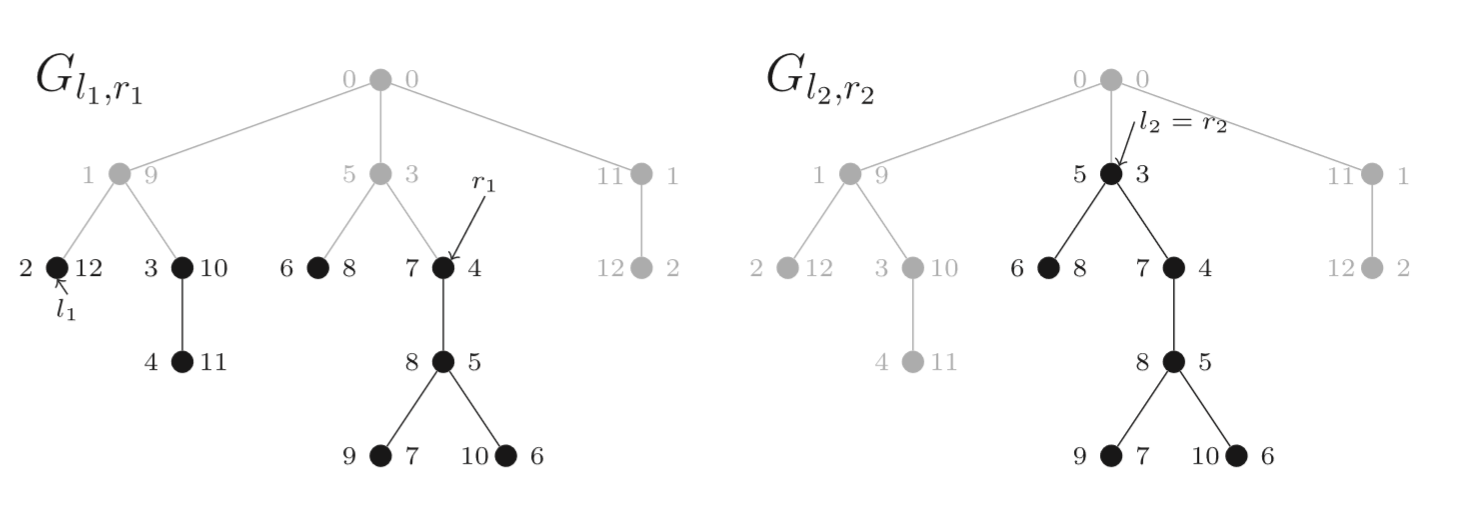
\includegraphics[width=14cm,clip]{Figures/RootEncoding}
		\label{Example subforests of tree G and their root encoding representation} 
		\caption{Example subforests of tree G and their root encoding representation~\cite{pawlik2015efficient}.}
\end{figure}
\subsection{Bottom-up Enumeration}
We presented the double root encoding for indexing sub-forests in the last section. In this section we make the use of this indexing scheme and present an algorithm for the enumeration of sub-forests pairs in bottom-up fashion.

The input of the algorithm are two trees $A$ and $B$ and a root-leaf path $\gamma$ of tree $A$. In algorithm 5, $p(v)$ is defined as the parent of the node $v$.
\IncMargin{1em}
\begin{algorithm}
  \caption{SUB\_FOREST\_PAIRS\_ENUMERATION}
  \SetKwInOut{Input}{inputs}
  \SetKwInOut{Output}{output}
  \SetKwData{TreeA}{$A$}
  \SetKwData{TreeB}{$B$}
  \SetKwData{RLP}{$\gamma$}
  \SetKwFunction{POSTORDER}{LR\_POSTORDER}{}{}

  \Input{\TreeA , \TreeB , \RLP}
  
  \ForEach{$node\ v\ \in\ \TreeA\ on\ the\ path\ from\ \epsilon\ to\ root$} { 
    $B' \gets B$\;
    $l_A^{last} \gets \varnothing$\;
    $l_A' \gets v$\;
  	\If{$\gamma\ is\ right\ or\ inner$} {
      \ForEach{$node\ r_B \in\ B\ in\ reverse\ right-to-left\ preorder$} { 
    	\If{$\gamma\ is\ right$} {   
    	  $l_A^{last} \gets p(v)$\;
    	  \lIf{$r_B\ is\ the\ rightmost\ child\ of\ its\ parent$} {
		     $B' \gets B(p(r_B))$  				
    	  }
    	  \lElse{
    		 $B' \gets \varnothing$
    	  }
    	  $r_A \gets v$\; 		
    	  }
    	  \ForEach{$node\ l_A \in\ left(A(p(v)), v) \cup l_A^{last}\ in\ reverse\ left-to-right\ preorder$} {
    	     \lIf{$l_A = p(v)$} {
			   $r_A \gets p(v)$				
    		  }
    		 \ForEach{$node\ l_B\ \in\ \{r_B\} \cup left(G, r_B)\ in\ reverse\ left-to-right\ preorder$} {
    			Compute forest-to-forest distance $d(l_A, r_A, l_B, r_B)$ as in Equation 2.3\;
    		  }
    		  $l_A' \gets l_A$\;
    		 }
    	  }	    	
    	}
     \If{$\gamma\ is\ left\ or\ inner$} {
     	\ForEach{$node\ l_B \in\ B\ in\ reverse\ right-to-left\ preorder$} {
     	  \If{$\gamma\ is\ left$} {
			\lIf{$l_B\ is\ the\ leftmost\ child\ of\ its\ parent$} {
			  $B' \gets B(p(l_B)$		
			}
			\lElse {
              $B' \gets \varnothing$		
			}
     	  }
     	  $l_A \gets l_A'$\;	
     	  \ForEach{$node\ r_A \in\ right(A(p(v)), v) \cup p(v)\ in\ reverse\ right-to-left\ preorder$} {
			\lIf{$r_A = p(v)$} {
				$l_A \gets p(v)$		
			}
			
			\ForEach{$node\ r_B \in\ l_B \cup right(B', l_B)\ in\ reverse\ right-to-left\ preorder$} {
				Compute forest-to-forest distance $d(l_A, r_A, l_B, r_B)$ as in Equation 2.3\;		
			}     	  
     	  }		     	
     	}
     }
    }
\end{algorithm}

The sub-problems are produced in nested loops and are nested as follows:$A(B(C(D)), B'(C'(D')))$. A relevant sub-forests pair is defined of the form $(l_A, r_A, l_B, r_B)$ using double roots encoding. Each loops enumerate one of these nodes. In the innermost loop, the distance for the relevant sub-forests pair is computed via Equation 2.2 and 2.3.

Loop A iterates bottom-up over the nodes of path $\gamma$ staring with a dummy leaf node $\epsilon$ which is appended to the leaf node of the path $\gamma$. The dummy is used for prevent the leaf node being treated as a special case. Figure 3.2 illustrates the order of processing nodes in loops A.

\begin{figure}
		\centering
		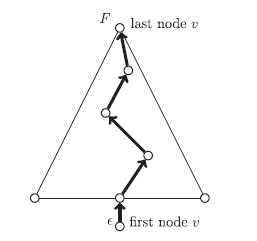
\includegraphics[width=4cm,clip]{Figures/loopA}
		\label{The order of processing nodes in loops A} 
		\caption{The order of processing nodes in loops A~\cite{pawlik2015efficient}.}
\end{figure}

Loop C enumerates the nodes to the left of path $\gamma$. The nodes set $left(A(p(v)), v)$ for a node enumerated in loop A is illustrated in Figure 3.3. Loop C(Figure 3.3(a)) defines the leftmost root node $l_A$ while the rightmost root node $r_A = v$ is defined by loop A. Symmetrically, loop C'(Figure 3.3(b)) iterates over the nodes from the set $right(A(p(v), v) \cup p(v)$ and defines the rightmost root node of the sub-forest, while the leftmost root node is the leftmost child of $p(v)$.

\begin{figure}
		\centering
		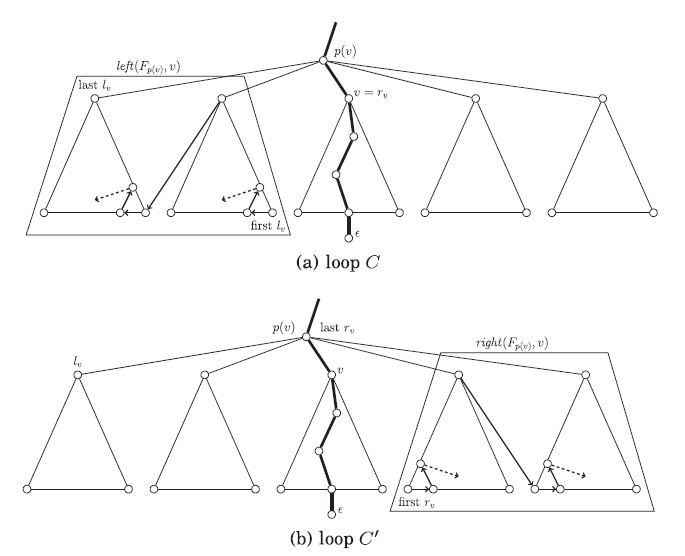
\includegraphics[width=10cm,clip]{Figures/loopCC}
		\label{The order of processing nodes in loop C and C'.} 
		\caption{The order of processing nodes in loop C and C'.~\cite{pawlik2015efficient}.}
\end{figure}

Loop B and loop D defines sub-forests of the tree $B$. The rightmost root node of sub-forest is iterates over all nodes of tree $B$ in reverse right-to-left preorder(Figure 3.4). After fixing the rightmost root node in loop B, the leftmost root node is iterated over all nodes to the left of leftmost root node in a specific sub-tree $B'$. 

\begin{figure}
		\centering
		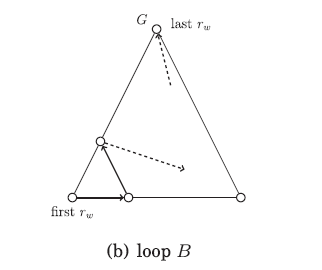
\includegraphics[width=6cm,clip]{Figures/loopB}
		\label{The order of processing nodes in loop B.} 
		\caption{The order of processing nodes in loop B.~\cite{pawlik2015efficient}.}
\end{figure}

\begin{figure}
		\centering
		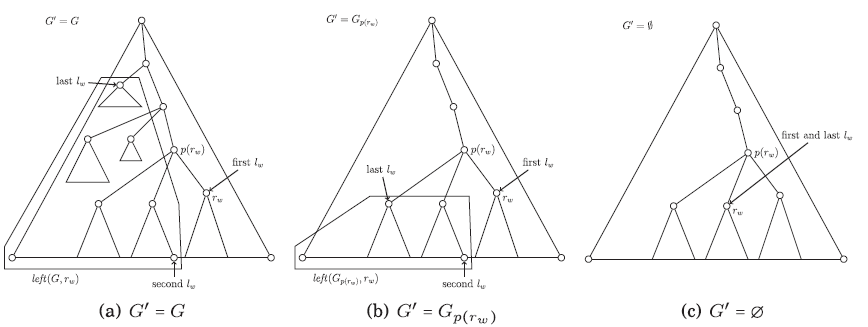
\includegraphics[width=14cm,clip]{Figures/loopD}
		\label{The order of processing nodes in loop D.} 
		\caption{The order of processing nodes in loop D.~\cite{pawlik2015efficient}.}
\end{figure}

The specific sub-tree $B'$ defines the set of nodes to be enumerated in loop D. The definition of $B'$ depends on the type of path $\gamma$ and the position of $r_B$ in B.
\begin{itemize}
\item Inner path $B' = B$(Figure 3.5(a))
\item Right path. If the rightmost root node $v$ is the rightmost child of its parent, then $B' = B(p(v))$(Figure 3.5(b)). Otherwise, $B' = \varnothing$(Figure 3.5(c)). 
\end{itemize}

Left paths are treated in loop B' and D', which are symmetric to loop B and D.

Algorithm 5 first enumerates the nodes to the left of the path then nodes to the right of the path in $A$. However, a symmetric version of Algorithm 5 goes on the other way: first iterates nodes to the right of the path then nodes to the right of the path. Since the directions of each nodes is not always the same, the symmetric version of  Algorithm 5 is included in our project as well.


\subsection{A Quadratic Space Complexity Implementation}
We have presented an algorithm for the enumeration of sub-forests pairs. It gives rise to two data structures:
\begin{itemize}
\item a permanent array D that stores the distance between a pair of sub-trees in two trees.
\item a temporary array F that stores the distance between a pair of sub-forests that are attached to the computation of a pair of sub-trees. 
\end{itemize}

Let $A$ and $B$ be two trees, and $\gamma$ be the root-leaf path on tree $A$. At the first glance, the array F requires cubic space, when the node on the root-leaf path is neither the leftmost child, nor the rightmost child, as the full decomposition of another tree is required in these cases.But it can be made quadratic with the introduction of two memorization tables: T and Q of sizes $\left\vert B \right\vert^2$ and $\left\vert A \right\vert$, where $A$ and $B$ are two trees.
\begin{itemize}
\item T stores the distance between a specific sub-forest in $A$ and each relevant sub-forests in $B$. 
\item Q stores the distance between each sub-forests of $A$ defined in loop C and a specific sub-forest in $G$, that is $G^{\comp}$
\end{itemize}

The tables T and Q are maintained in each loops C and C', which are needed in different calls of loops A and loops B(B').  In each loops A and B(B'), the intermediate results computed in the last loops are retrieved and is used for computation. Then, the new results are updated in T and Q for the next loop.

We now show how to retrieve intermediate result with the help of memorization tables $T$ and $Q$. Before we introduce rules for obtaining the required distances when computing each pairs of relevant sub-forest, it is beneficial to recall the formula used to compute the distance of relevant sub-forest pairs. If double roots encoding scheme is applied to index forests, the Equation 2.2 will change to Equation 3.1 an 3.2.

Let $A$ and $B$ be two trees.

\begin{equation}
d(A_{lA, rA}, B_{lB, rB}) = min \begin{cases}
d(A_{lA, rA} - lA, B_{lB, rB}) + \delta(lA, \varnothing)\\
d(A_{lA, rA}, B_{lB, rB} - lB) + \delta(\varnothing, lB)\\
d(A_{lA, rA} - A(lA), B_{lB, rB} - B(lB)) + d(A(lA), B(lB))\\
 \end{cases}
\end{equation}

Symmetrically, if right decomposition applied to the forests, the equation changes to 

\begin{equation}
d(A_{lA, rA}, B_{lB, rB}) = min \begin{cases}
d(A_{lA, rA} - rA, B_{lB, rB}) + \delta(rA, \varnothing)\\
d(A_{lA, rA}, B_{lB, rB} - rB) + \delta(\varnothing, rB)\\
d(A_{lA, rA} - A(rA), B_{lB, rB} - B(rB)) + d(A(rA), B(rB))\\
\end{cases}
\end{equation}
 
As can be seen in the Equation 3.1, four intermediate results are needed to retrieve in each recursive calls, $d(A_{lA, rA} - lA, B_{lB, rB})$, $d(A_{lA, rA}, B_{lB, rB} - lB)$, $d(A(lA) - lA, B(lB) - lB)$ and $d(A_{lA, rA} - A(lA), B_{lB, rB} - B(lB))$ respectively. Please note that we only consider the left decomposition for the right decomposition case is symmetric.

\begin{equation}
d(A_{lA, rA} - lA, B_{lB, rB}) = \begin{cases}
\sum_{v \in B_{lB, rB}} \delta(\varnothing, v)\ if\ A_{lA, rA} - lA = \varnothing \\
T[lB, rB]\ if\ A_{lA, rA} - lA\ is\ a\ tree\\
F[a, lB]\ otherwise
\end{cases}
\end{equation}
Note: $a \in A$ such that $A_{a, rA} = A_{lA, rA} - lA$
\begin{equation}
d(A_{lA, rA}, B_{lB, rB} - lB) = \begin{cases}
\sum_{v \in A_{lA, rA}} \delta(v, \varnothing)\ if\ B_{lB, rB} - lB = \varnothing \\
Q[lA]\ if\ B_{lB, rB}\ is\ a\ tree\\
F[l_A, b]\ otherwise
\end{cases}
\end{equation}
Note: $b \in B$ such that $B_{b, rB} = B_{lB, rB} - lB$
\begin{equation}
d(A(lA), B(lB)) = \begin{cases}
\sum_{v \in B(lB)} \delta(\varnothing, v)\ if\  A_{lA, rA} - lA = \varnothing \\
\sum_{v \in A(lA)} \delta(v, \varnothing)\ if\ B_{lB, rB} - lB = \varnothing \\
D[lA, lB]\ otherwise  
\end{cases}
\end{equation}
\begin{equation}
d(A_{lA, rA} - A(lA), B_{lB, rB} - B(lB)) = \begin{cases}
0\ if A_{lA, rA} - A(lA) \cap B_{lB, rB} - B(lB) = \varnothing \\
\sum_{v \in B_{lB, rB} - B(lB)} \delta(\varnothing, v)\ if A_{lA, rA} - A(lA) = \varnothing \\
\sum_{v \in A_{lA, rA} - A(lA)} \delta(v, \varnothing)\ if B_{lB, rB} - B(lB) = \varnothing \\
T[y, rB]\ if A_{lA, rA} - A(lA)\ is\ a\ tree\\
F[x, y]\ otherwise\\
\end{cases}
\end{equation}
Note: $x \in A$, such that $A_{x, rA} = A_{lA, rA} - A(lA)$, $y \in B$, such that $B_{y, rB} = B_{lB, rB} - B(lB)$.

\doublespacing
\chapter{Another algorithmic improvement}
An algorithmic improvement can be applied to our algorithm. 
\section{Main Idea}
We notice that a large number of non-branching nodes exist in the tree representation of the RNA secondary structure. Therefore, we can construct compact representation for trees, which can aid in improving the running time for computing the tree edit distance. 
\section{Vertical Reduction on Trees}
Before we introduce the reduction on trees, it is benefit to define the compressible path on trees.
\begin{definition}
(Maximal Non-branching Path)A path in a tree is a non-branching path
if both the post-order tree traversal and pre-order tree traversal visit the nodes on the path in consecutive order. A non-branching path is maximal if no other non-branching path contains it ~\cite{Chen2014}.
\end{definition}

\begin{figure}
		\centering
		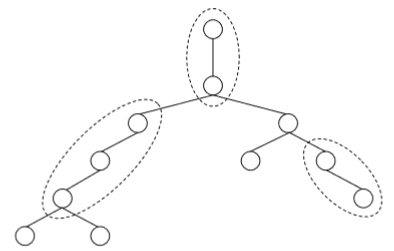
\includegraphics[width=6cm,clip]{Figures/VComponent}
		\label{Maximal Non-branching Path.} 
		\caption{Maximal non-branching path ~\cite{Chen2014}.}
\end{figure}
Figure 4.1 is an example of maximal non-branching path. Each maximal non-branching paths is enclosed by dashed line.

Each maximal non-branching paths is compressible, which gives rise to the vertical reduction.
\begin{definition}
(Vertical Reduction)
The vertical reduction on a tree is to replace every maximal non-branching path in the tree by a single node~\cite{Chen2014}.
\end{definition}

\begin{figure}
		\centering
		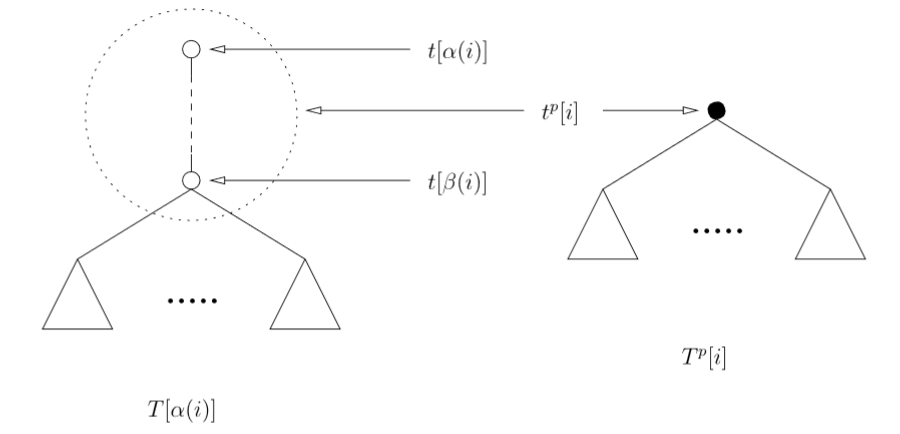
\includegraphics[width=10cm,clip]{Figures/VReduction}
		\label{An Example of the Mapping of Nodes Between the Original Tree and its Vertical Reduced Tree} 
		\caption{An example of the mapping of nodes between the original tree and its vertical reduced tree ~\cite{Chen2014}.}
\end{figure}

In Figure 4.2, we give an example of the mapping of nodes between the original tree(n the left) and its tree(on the right). Given a vertical reduced tree $\widetilde{T}$, two functions are respectively defined to map a node in compressed tree $\widetilde{t}[i]$ to the highest indexed node in the original tree $T$ $t[\alpha(i)]$ and the lowest indexed node $t[\beta(i)]$ of in the original tree $T$.  When $\widetilde(t)[i]$ corresponds to a single node in T, $t[\alpha(i)]=t[\beta(i)]$.

Please note that the compressed tree is just a compact representation of the original. Therefore, the strategy-based strategy in chapter 4 applied to the compressed tree can get the result same as that applied to the original tree. In other words, given trees $(T_1, T_2)$ and their reduced tree$(\widetilde{T_1}, \widetilde{T_2})$, the relation $d(\widetilde{T_1}, \widetilde{T_2}) = d(T_1, T_2)$ is implied. 

\section{Computation}

Following the Equation 2.3, let $\widetilde{F_1}$ and $\widetilde{F_2}$ be two relevant sub-forests in compressed trees,  $u$ and $v$ are nodes in forests $\widetilde{F_1}$ and $\widetilde{F_2}$ respectively, the forest-to-forest distance can be computed as follows:
\begin{equation}
d(\widetilde{F_1}, \widetilde{F_2}) = min \begin{cases}
d(\widetilde{F_1} - u, \widetilde{F_2}) + \delta(u, \varnothing) \\
d(\widetilde{F_1}, \widetilde{F_2} - v) + \delta(\varnothing, v) \\
d(\widetilde{F_1} - \widetilde{F_1(u)}, \widetilde{F_2} - \widetilde{F_2(v)}) + d(\widetilde{F_1(u)}, \widetilde{F_2(v)}) 
\end{cases}
\end{equation}
Each pairs of forest-forest distance $d(\widetilde{F_1}, \widetilde{F_2})$ can be computed correctly since each sub-problems has already been computed beforehand if implemented in post-order. The tree-tree distance, $d(\widetilde{F_1(u)}, \widetilde{F_2(v)})$, however, have never been computed before and must compute its value.

The tree-tree distance in compressed tree can be computed in the following lemmas.

\begin{lemma}
$d(\widetilde{F_1(i)}, \widetilde{F_2(j)}) = d(F_1(\alpha(i), F_2(\alpha(j))))$, where $i$ is a node in $\widetilde{F_1}$ and $j$ is a node in $\widetilde{F_2}$
\end{lemma}
\begin{proof}
The result follows from the compressed tree definition and the post-order implementation.
\end{proof}

To compute tree-to-tree distance of each sub-trees pairs in original trees, following Equation 2.2, we have Equation 4.2.

\begin{lemma}
$\forall u \in \{\beta(i), \cdots, \alpha(i)\}$ where $i$ is a node in $\widetilde{F_1}$, and $\forall v \in \{\beta(j), \cdots, \alpha(j)\}$ where $j$ is a node in $\widetilde{F_2}$.
\begin{equation}
d(F_1(u), F_2(v)) = min\begin{cases}
d(F_1^{\comp}(u), F_2(v)) + \delta(u, \varnothing)\\
d(F_1(u), F_2^{\comp}(v)) + \delta(\varnothing, v)\\
d(F_1^{\comp}(u), F_2^{\comp}(v)) + \delta(u, v)
\end{cases}
\end{equation}
\end{lemma}
\begin{proof}
The known recursive solution for the tree-to-tree edit distance.
\end{proof}

The computation of $d(F_1(u), F_2(v))$ involves sub-problems $d(F_1(u), F_2^{\comp}(\beta(j))), \forall u \in \{\beta(i), \cdots, \alpha(i)\}$ and $d(F_1^{\comp}(\beta(i)), F_2(v)), \forall v \in \{\beta(i), \cdots, \alpha(i)\}$ for the first time and therefore must compute their values beforehand. Therefore, initialization should be done to compute these values.  


\begin{lemma}
Let $F_2^{\comp}(\beta(j))$ be the form $F_2(j_1) \comp F_2(j_2) \cdots F_2(j_l)$, where $j \in \widetilde{F_2}$ and $j_1, j_2, \cdots, j_l$ be children of node $j$, $\forall u \in \{\beta(i), \cdots \alpha(i)\}$, where $i \in \widetilde{F_1}$,
\begin{equation}
d(F_1(u), F_2^{\comp}(\beta(j))) = min \begin{cases}
d(F_1^{\comp}(u), F_2^{\comp}(\beta(j))) + \delta(u, \varnothing)\\
min_{j_1' \leq q \leq j_l}\{d(F_1(u), F_2(\alpha(q))) - d(\varnothing, F_2(\alpha(q)))\} + d(\varnothing, F_2^{\comp}(\beta(j)))
\end{cases}
\end{equation}
\end{lemma}
\begin{proof}
The edit distance between tree $F_1(u)$ and the forest $F_2^{\comp}(\beta(j))$ consists of two possible cases. In the first case, $u$ is constrained to be deleted and the remaining substructure $F_1^{\comp}(u)$ is matched to $F_2^{\comp}(\beta(j))$. In the second case, $u$ is constrained to match a node somewhere in $F_2^{\comp}(\beta(j))$. In other words, tree $F_1(u)$ is matched to a sub-tree in $F_2^{\comp}(\beta(j))$. Therefore, the second case is finding a sub-tree in $F_2^{\comp}(\beta(j))$ to be matched to $F_1(u)$ so as to minimize $d(F_1(u), F_2^{\comp}(\beta(j)))$ under such constraint. 
\end{proof}

\begin{lemma}
Let $F_1^{\comp}(\beta(i))$ be the form $F_1(i_1) \comp F_1(i_2) \cdots F_1(i_k)$, where $i \in \widetilde{F_1}$ and $i_1, i_2, \cdots, i_l$ be children of node $i$, $\forall v \in \{\beta(j), \cdots \alpha(j)\}$, where $j \in \widetilde{F_2}$,
\begin{equation}
d(F_1^{\comp}(\beta(i)), F_2(v)) = min \begin{cases}
d(F_1^{\comp}(\beta(i)), F_2^{\comp}(v)) + \delta(\varnothing, v)\\
min_{i_1 \leq p \leq i_k}\{d(F_1(\alpha(p)), F_2(v)) - d(F_1(\alpha(p)), \varnothing)\} + d(F_1^{\comp}(\beta(i)), \varnothing)
\end{cases}
\end{equation}
\end{lemma}
\begin{proof}
The proof of Lemma 4.3.4 is symmetric to that of Lemma 4.3.3. The edit distance is the minimum value under two categories of constraints. 
\end{proof}

\section{Implementation}
The compressed tree is just a compact representation of the original. Thus, the algorithm is the same as in the Chapter 3:first find the optimal root-leaf path in compressed trees then compute distance in the bottom-up fashion. By Equation 4.1 and Lemma 4.3.1, 4.3.2, 4.3.3, the tree edit distance computation on compressed trees makes no differences to that on original trees when computing forest-to-forest distance but requires extra initialization steps when computing tree-to-tree distance. 

The tree-to-tree edit distance gives rise to five data structures. Let $T_1$ and $T_2$ be two original trees, while $\widetilde{T_1}$ and $\widetilde{T_2}$ be two compressed trees after vertical reductions on tree $T_1$ and $T_2$ respectively.
\begin{itemize}
\item $D_t$: a two dimensional permanent array of size $(\left\vert T_1 \right\vert + 1) * (\left\vert T_2 \right\vert + 1)$, which is used to store distance with respect to the $(T_1, T_2)$ representation.
\item $\widetilde{D_t}$: a two dimensional permanent array of size $(\left\vert \widetilde{T_1 }\right\vert + 1) * (\left\vert \widetilde{T_2} \right\vert + 1)$, which is used to store distances with respect to the $(\widetilde{T_1}, \widetilde{T_2})$ representation. 
\item $\widetilde{D_f}$: a two dimensional temporary array of size $(\left\vert \widetilde{T_1 }\right\vert + 1) * (\left\vert \widetilde{T_2} \right\vert + 1)$, which is used to store intermediate results for forest-to-forest distances.
\item $A_1, A_2$: temporary one dimensional arrays of lengths $(\left\vert T_1 \right\vert + 1)$ and $(\left\vert T_2 \right\vert + 1)$ respectively, which is used handle boundary initialization. 
\end{itemize}

We now present the algorithms to compute tree-to-tree edit distance on compressed trees. The algorithm details are shown in Algorithm 6. Let $\widetilde{A}$ and $\widetilde{B}$ be two compressed trees, $i \in \widetilde{A}$ and $j \in \widetilde{B}$.

\IncMargin{1em}
\begin{algorithm}
  \caption{TREE\_TO\_TREE\_DISTANCE}
  \SetKwData{TreeA}{$\widetilde{A(i)}$}
  \SetKwData{TreeB}{$\widetilde{B(j)}$}

  \For{$u \gets \beta(i) - 1$ \KwTo $\alpha(i)$} {
	$A_1[u] \gets D_t[u, \beta(j) - 1]$\;  
  }
  \For{$v \gets \beta(j)$ \KwTo $\alpha(j)$} {
	$A_2[v] \gets D_t[\beta(i) - 1, v]$\;  
  }
  $D_t[\beta(i) - 1, \beta(j) - 1] \gets \widetilde{D_f}[i - 1, j - 1]$\;
  \For{$u \gets \beta(i)$ \KwTo $\alpha(i)$} {
	$D_t[u, \beta(j) - 1] \gets min \begin{cases}
	D_t[u - 1, \beta(j) - 1] + \delta(A[u], \varnothing)\\
	min_{j_1 \leq q \leq j_l}\{D_t[u, \alpha(q)] - \sum_{k \in B(\alpha(q))}\delta(\varnothing, k)\} + \sum_{k \in B(\beta(j))}\delta(\varnothing, k)
	\end{cases}	
	$  
  }
  \For{$v \gets \beta(j)$ \KwTo $\alpha(j)$} {
  	$D_t[\beta(i) - 1, v] \gets min \begin{cases}
  	D_t[\beta(i) - 1, v - 1] + \delta(\varnothing, B[v])\\
  	min_{i_1 \leq p \leq i_k}\{D_t[\alpha(p), v] - \sum_{k \in A(\alpha(p))}\delta(k, \varnothing)+ \sum_{k \in A(\beta(i))}\delta(k, \varnothing)\}
	\end{cases}  	
  	$
  }
  \For{$u \gets \beta(i)$ \KwTo $\alpha(i)$} {
	\For{$v \gets \beta(j)$ \KwTo $\alpha(j)$} {
		$D_t[u, v] \gets min \begin{cases}
		D_t[u - 1, v] + \delta(u, \varnothing)\\
		D_t[u, v - 1] + \delta(\varnothing, v)\\
		D_t[u - 1, v - 1] + \delta(u, v)
		\end{cases}		
		$	
	} 
  }
  $\widetilde{D_t}[i, j] \gets D_t[\alpha(i), \alpha(j)]$\;
  $\widetilde{D_f}[i, j] \gets D_t[\alpha(i), \alpha(j)]$\;
  \For{$u \gets \beta(i) - 1$ \KwTo $\alpha(i)$}{
  	$D_t[u, \beta(j) - 1] \gets A_1[u]$\;
  }
  \For{$v \gets \beta(j)$ \KwTo $\alpha(j)$} {
	$D_t[\beta(i) - 1, v] \gets A_2[v]$\;  
  }
\end{algorithm}

The algorithm of forest-to-forest edit distance on compressed trees is the exactly the same as that on original trees, using Equation 3.1 or 3.2 depending on the decomposition directions. The details of the forest-to-forest edit distance computation is shown in Algorithm 7 and 8.

\IncMargin{1em}
\begin{algorithm}
  \caption{FOREST\_TO\_FOREST\_DISTANCE}
  \SetKwData{TreeA}{$\widetilde{A(i)}$}
  \SetKwData{TreeB}{$\widetilde{B(j)}$}
  $sizelA \gets$ the size of A(lA)\;
  $sizelB \gets$ the size of B(lB)\;
  $\widetilde{D_f}[lA, lB] \gets min \begin{cases}
	\widetilde{D_f}[lA - 1, lB] + \delta(lA, \varnothing)\\
	\widetilde{D_f}[lA, lB - 1] + \delta(\varnothing, lB)\\
	\widetilde{D_f}[lA - sizelA, lB - sizelB] + \widetilde{D_t}[lA, lB]
  \end{cases}  
  $
\end{algorithm}

\IncMargin{1em}
\begin{algorithm}
  \caption{FOREST\_TO\_FOREST\_DISTANCE}
  \SetKwData{TreeA}{$\widetilde{A(i)}$}
  \SetKwData{TreeB}{$\widetilde{B(j)}$}
  $sizerA \gets$ the size of A(rA)\;
  $sizerB \gets$ the size of B(rB)\;
  $\widetilde{D_f}[rA, rB] \gets min \begin{cases}
	\widetilde{D_f}[rA - 1, rB] + \delta(rA, \varnothing)\\
	\widetilde{D_f}[rA, rB - 1] + \delta(\varnothing, rB)\\
	\widetilde{D_f}[rA - sizerA, lB - sizerB] + \widetilde{D_t}[rA, rB]
  \end{cases}  
  $
\end{algorithm}
\doublespacing
\chapter{Experiment}
We describe an application which would benefit from our algorithm, namely RNA secondary structure comparison. 

\section{RNA and its Secondary Structure}
RNA is an essential molecule in organisms which has a wide range of functions in biological systems.Cellular organisms use messenger RNA (mRNA) to convey genetic information (using the letters G, U, A, and C to denote the nitrogenous bases guanine, uracil, adenine, and cytosine) that directs synthesis of specific proteins. Besides, many viruses encode their genetic information using an RNA genome.

RNA is assembled as a chain of nucleotides, but unlike DNA it is more often found in nature as a single-strand folded onto itself, rather than a paired double-strand. However, it can fold back onto itself by means of hydrogen bonding between distant complementary nucleotides(A=U, G$\equiv$C), resulting in the secondary structure. We define the secondary structure of RNA as follows.

\begin{definition}
(RNA secondary structure) A secondary structure is primarily a list of base pair $\omega$. A valid secondary structure should satisfy the following constraints:
\begin{itemize}
\item A base cannot participate in more than one base pair, i.e., $\omega$ is a matching on the set of sequence positions.
\item No two base pairs $(i, j)$ and $(k, l)$ $\in \omega$ "cross" in the sense that $i < k < j < l$.
\end{itemize}
\end{definition}

The first condition excludes tertiary structure motifs such as base triplets while the second condition avoid the pseudo knot in RNA structures. However, the fact is that pseudo knots do occur in RNA structures, namely RNA tertiary structure. To simplify, we don't consider the tertiary structure of RNA in this experiment and assume that any nucleotide participates in at most one such pair and the bonded pairs are non-crossing. 

Figure 5.1 is an example of invalid RNA structure in our experiment, which has tertiary structures(marked in dotted blue lines) and base triplets.
\begin{figure}
		\centering
		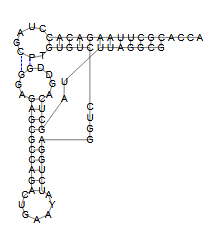
\includegraphics[width=5cm,clip]{Figures/RNATT}
		\label{RNA Tertiary Structure.} 
		\caption{RNA Tertiary Structure.}
\end{figure}
\section{String Representation of the RNA Secondary Structure}
Secondary structure can also been stored compactly in strings consisting of dots and matching brackets:For any pair between positions i and j $(i < j)$ we place an open bracket "(" at position i and a closed bracket ")" at j, while unpaired positions in the molecule are represented by a dot ".".Figure 5.2 illustrates the string presentation with dots and brackets of the RNA secondary structure. 

\begin{figure}
		\centering
		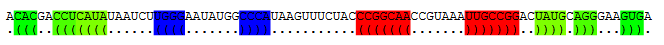
\includegraphics[width=18cm,clip]{Figures/RNAST1}
		\label{String Representation of the RNA Secondary Structure.} 
		\caption{String representation of the RNA secondary structure.}
\end{figure}
\section{RNA Secondary Structure Graphs}
Secondary structures can be represented by "secondary structure graphs". According the base pair information in Figure 5.2, the string can be fold into a circle(Figure 5.3 on the left) or a secondary structure graph(Figure 5.3 on the right).

\begin{figure}
		\centering
		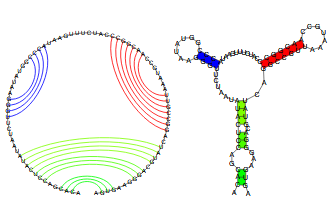
\includegraphics[width=10cm,clip]{Figures/RNAST2}
		\label{Graph Representation of the RNA Secondary Structure.} 
		\caption{Graph representation of the RNA secondary structure.}
\end{figure}

\section{Tree Representation of the RNA Secondary Structure}
In the computer science point of view, the secondary structure of an RNA molecule can be topologically represented by a tree. As shown in Figure 5.2, the RNA secondary structure graphs consists of two distinct category of nucleotides: those that are interacting via hydrogen bonding (so called stems), and those that are not(so call loops). Stems and loops in RNA can be represented as nodes in a tree. Leaves may be labeled with the corresponding unpaired base, while interior nodes are labeled with the corresponding base pair. To make things simplifier, we use different characters apart from alphabet$\{A, U, G, C\}$ to labeled each base pairs. Table 5.1 illustrates the label of each base pairs. 
\begin{table}
			\centering
			\begin{tabular}{l l}
				\toprule
				\textbf{Base Pairs} & \textbf{Label}\\
				\midrule
				$A = U$ & F\\
				$G \equiv C$ & J\\
				$U = A$ & P\\
				$C \equiv G$ & M\\
			\end{tabular}
		\caption{The Label of Base Pair}
\end{table}
In this way,the RNA secondary structure can be converted into a tree. Figure 5.4 is the corresponding tree representation of the secondary structure of RNA in Figure 5.3.

\begin{figure}
		\centering
		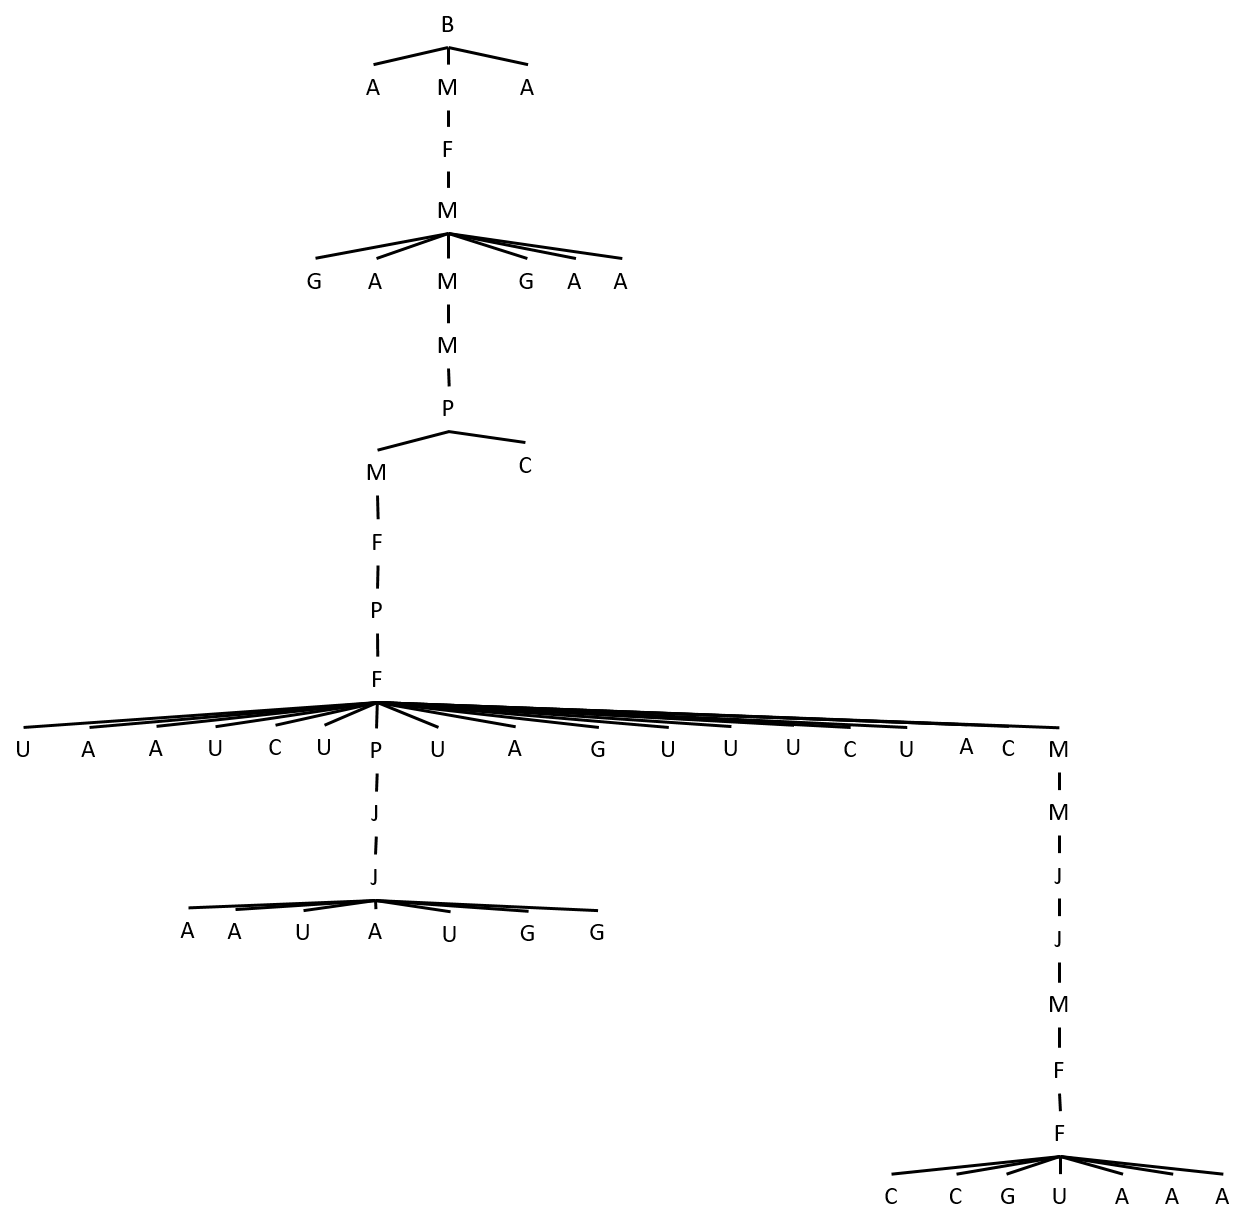
\includegraphics[width=16cm,clip]{Figures/RNAST3}
		\label{Tree Representation of the RNA Secondary Structure.} 
		\caption{Tree representation of the RNA secondary structure.}
\end{figure}

\section{Datasets}
We grab RNA data from the Ribonuclease P Database~\cite{brown1998ribonuclease}. The database consists of a compilation of RNase P sequences, sequence alignments, secondary structures,  three-dimensional models and accessory information as well. The data can be downloaded from the website
\url{http://www.mbio.ncsu.edu/RNaseP/home.html}.

The RNA files in the database are stored in XML format. The RNA files consist of RNA names, description, sequences as well as secondary structure base pairs.
Figure 5.4 is an example of RNA files in the database. The RNA name is "A.tumefaciens RNase P RNA" with the length 402 nt. These two information are included between tags. The following information is the RNA sequence. The RNA second structure information is stored in base pairs indexed by the position in the RNA sequence. Each lines has two base indexes, meaning that two nucleotides are binding to each other. 
\begin{figure}
		\centering
		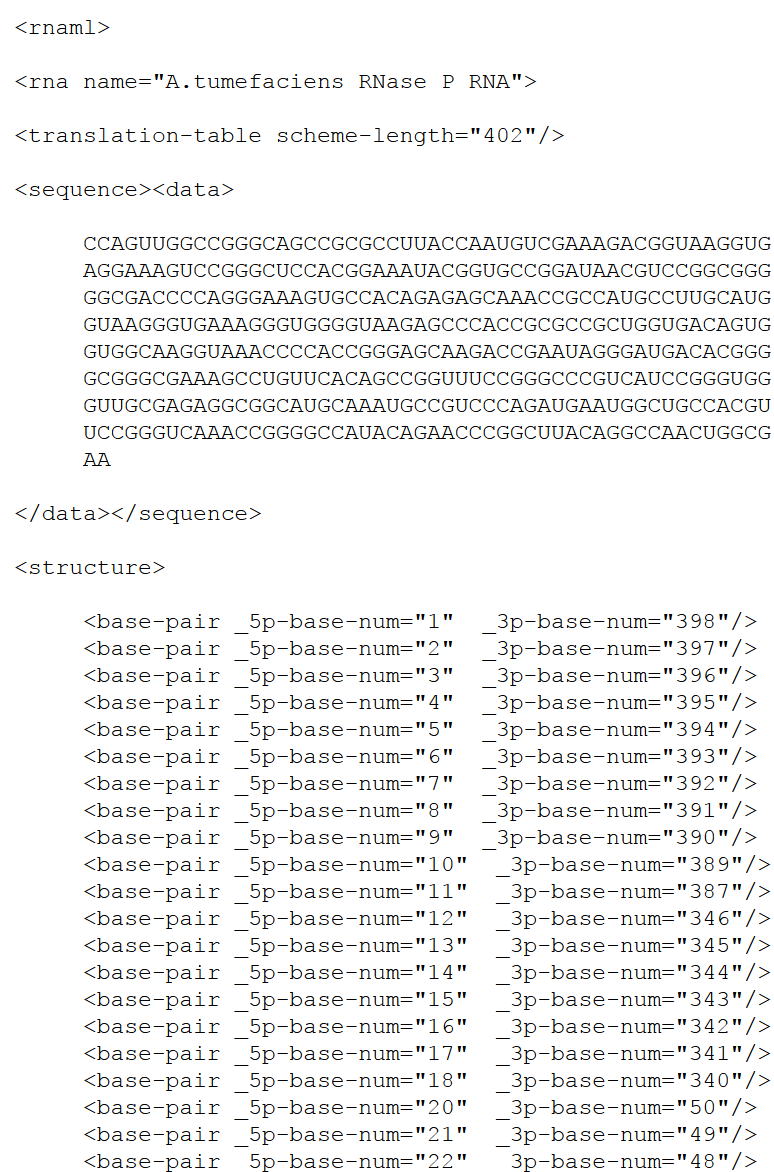
\includegraphics[width=13cm,clip]{Figures/RNADatabase}
		\label{An RNA Sequence in XML Format.} 
		\caption{An RNA Sequence in XML Format.}
\end{figure}

We use the information from RNA files to construct trees. Then the problem of comparing the similarity between two RNA secondary structures becomes comparing the edit distance between two trees. Our algorithms in Chapter 3 and 4 can help solve the problem. 

Another dataset we use in our experiments 

\section{Some Experimental Result}
In our experiments, we compute alignments between RNA secondary structure from Ribonuclease P Database. Figures 5.6 and 5.7 show two RNA structures in string representation. On the other hand, the corresponding graph representations are shown in Figures 5.8 and 5.9. We notice that the raw data contains tertiary structures. Therefore, we first remove the tertiary structures before constructing the corresponding tree data structure. Figure 5.10 shows the alignment results where the cost of each valid operation(deletion, insertion and substitution) is 1.

\begin{figure}
		\centering
		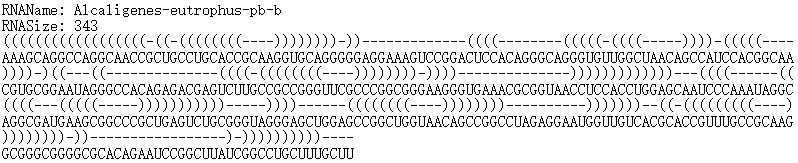
\includegraphics[width=17cm,clip]{Figures/AlcaligenesString}
		\label{Alcaligenes eutrophus Sequence from the RNase P database.} 
		\caption{Alcaligenes eutrophus Sequence from the RNase P database.}
\end{figure}

\begin{figure}
		\centering
		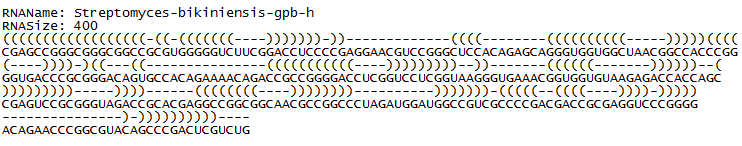
\includegraphics[width=17cm,clip]{Figures/StreptomycesString}
		\label{Streptomyces bikiniensis Sequence from the Rnase P database.} 
		\caption{Streptomyces bikiniensis Sequence from the RNase P database. }
\end{figure} 

\begin{figure}
		\centering
		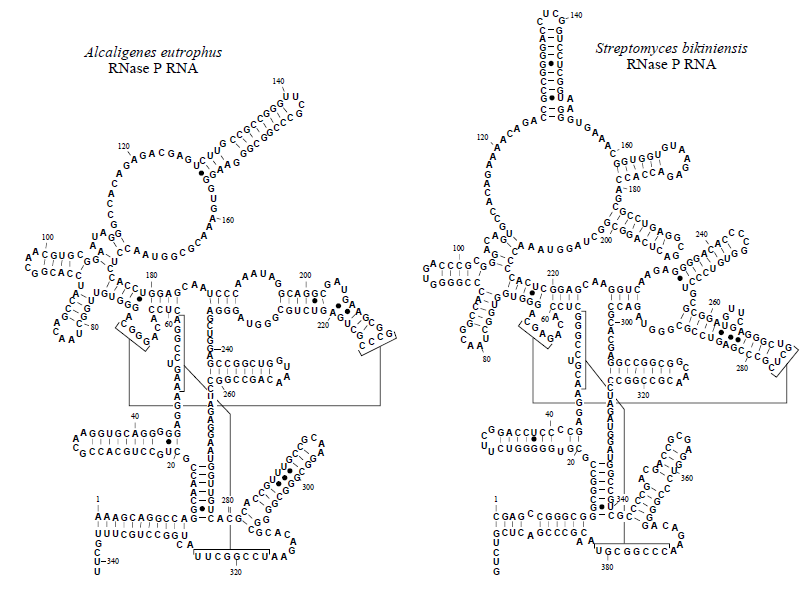
\includegraphics[width=13cm,clip]{Figures/RNAGraphExample}
		\label{The structures of RNase P RNA of Cupriavidus metallidurans (Alcaligenes eutrophus) and Streptomyces bikiniensis.} 
		\caption{The structures of RNase P RNA of Cupriavidus metallidurans (Alcaligenes
eutrophus) and Streptomyces bikiniensis.}
\end{figure}

\begin{figure}
		\centering
		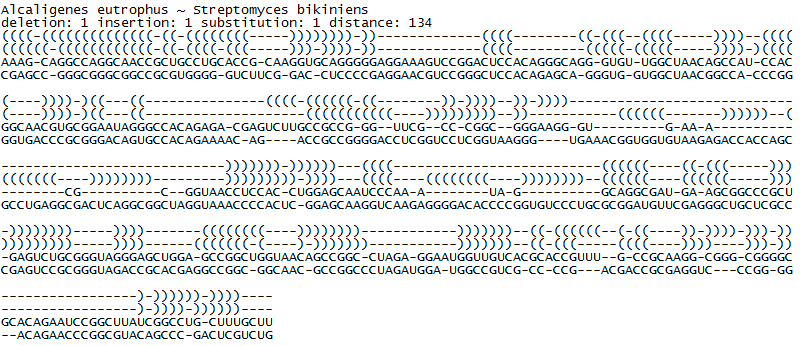
\includegraphics[width=17cm,clip]{Figures/AlignmentResult}
		\label{Alignment Between Two RNAs.} 
		\caption{Alignment Between the Secondary Structure of Alcaligenes eutrophus and Streptomyces bikiniensis.}
\end{figure}

We run our program on larger RNA sequences as well. We compare the edit distance between 2 rRNAs from two organism named "Marchantia polymorpha Chloroplast" and "Archaeoglobus fulgidus". Both of them have the length over 1000 nucleotides. The test result when the cost of each valid operations is 1 is shown in Figure 5.10. 

\section{Evaluation}
We empirically evaluate our algorithm with other four state-of-the-art algorithms on Ribonuclease P Database and compare the relevant sub-problems and actual run time to the algorithms proposed in Chapter 2: the algorithm by Zhang and Shasha and its symmetric version always using right paths~\cite{zhang1989simple}. All algorithms are implemented as single-thread applications in C++ and run on a 64-core 3.4GHZ Ubuntu. The source code is available online.

Firstly we compare the number of relevant sub-problem computed by each of the algorithms for a pair of specific RNA secondary structures. Each relevant sub-problems are the constant-time operations that make up the complexity of the algorithm. Then, we mark the actual run time of each algorithms. The evaluation results are shown in Table 5.2 and 5.3. As according to our test results, our decomposition strategies on compressed trees is the best strategies compared to other methods, creating the least number of relevant sub-problems. 

\begin{table}
			\centering
			\begin{tabular}{l l l}
				\toprule
				\textbf{Algorithm} & \textbf{$\#Rel.sub$} &\textbf{Time[sec]}\\
				\midrule
				$Zhang-L$ & 849282 & 0.08\\
				$Zhang-R$ & 2039089 & 0.13\\
				$Our\ Algorithm(Before\ Compression)$ & 553526 & 0.04\\
				$Zhang-L(Compressed)$ & 428766 & 0.05\\
				$Zhang-R(Compressed)$ & 686562 & 0.05\\
				$Our\ Algorithm(After\ Compression)$ & 291329 & 0.03\\
			\end{tabular}
		\caption{The Relevant Sub-problem and its Actual Run Time of Each Algorithms}
\end{table}

\begin{table}
			\centering
			\begin{tabular}{l l l}
				\toprule
				\textbf{Algorithm} & \textbf{$\#Rel.sub$} &\textbf{Time[sec]}\\
				\midrule
				$Zhang-L$ & 41889364 & 3.2\\
				$Zhang-R$ & 42972591 & 3.3\\
				$Our\ Algorithm(Before\ Compression)$ & 32254346 & 2.3\\
				$Zhang-L(Compressed)$ & 17769036 & 0.47\\
				$Zhang-R(Compressed)$ & 18154025 & 0.51\\
				$Our\ Algorithm(After\ Compression)$ & 13546825 & 0.34\\
			\end{tabular}
		\caption{The Relevant Sub-problem and its Actual Run Time of Each Algorithms}
\end{table}




\begin{figure}
		\centering
		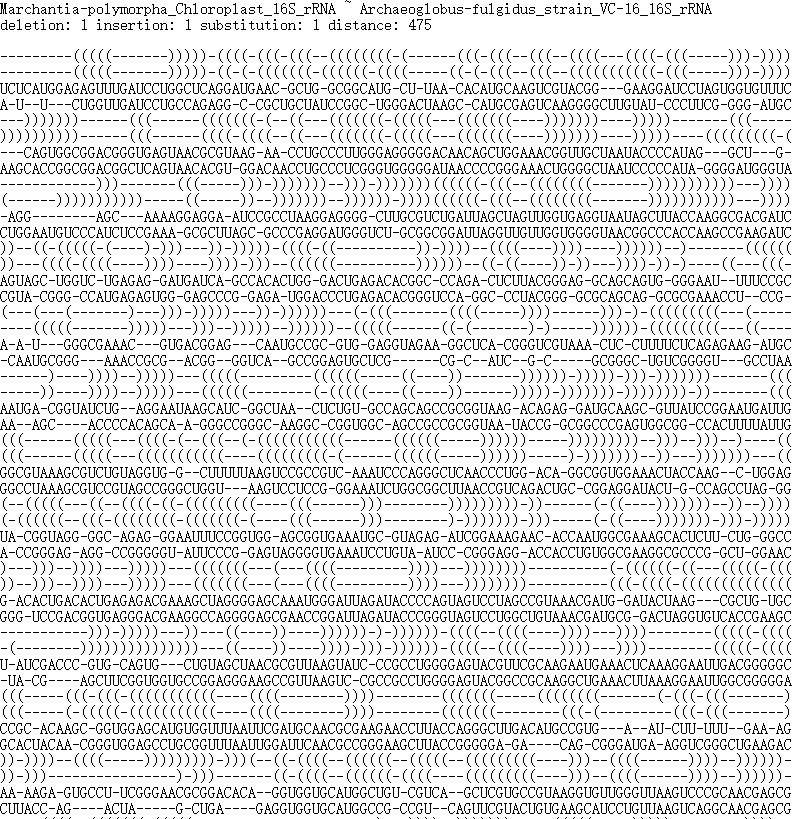
\includegraphics[width=17cm,clip]{Figures/AlignmentResult2}
		\label{Alignment Between Two RNAs.} 
		\caption{Alignment Between the Secondary Structure of rRNA from Marchantia polymorpha Chloroplast and Archaeoglobus fulgidus.}
\end{figure}




\doublespacing
\chapter{Conclusion}
In this thesis, we have studied the topic of tree edit distance computation. After the definition of tree edit distance, we have given an overview of existing approaches for tree edit distance and their decomposition strategies, including leftmost paths decomposition, rightmost paths decomposition, heavy path decomposition on one tree and that on both trees as well. These methods take advantage of the overlap among sub-forests that are contained in the same sub-tree, and the overlap of sub-trees in different ways. 

We proposed a new algorithm to find the optimal root-leaf path decomposition that avoid redundant computation. The algorithm uses dynamic programming and is implemented using C++. An overview description and some detailed implementations have been illustrated in Chapter 2.

Another algorithmic improvement can be applied to our algorithm to reduce time complexity. We compressed the non-branching nodes to a single node to compress tree in the vertical direction. After the vertical reduction, the compressed trees then are used for computation. The detailed implementations are shown in Chapter 3.

RNA secondary structure similarity comparison is an application of our algorithm. We test our algorithm on the Ribonuclease P Database and evaluation the time complexity by counting the relevant sub-problem and mark the actual run time. According the test result, our algorithm is by far the best decomposition strategy for trees. 
 
A lot of research remains to be done. Our results are good but we hope to improve them. 


%% This adds a line for the Bibliography in the Table of Contents.
\addcontentsline{toc}{chapter}{Bibliography}
%% ***   Set the bibliography style.   ***
\bibliographystyle{plain} % (change according to your preference)
%%% ***   Set the bibliography file.   ***
\bibliography{westernthesis}{}
%% ***   NOTE   ***
%% If you don't use bibliography files, comment out the previous line
%% and use \begin{thebibliography}...\end{thebibliography}.  (In that
%% case, you should probably put the bibliography in a separate file
%% and \include or \input it here).

%Appendices.
%\begin{appendices}
%\chapter{Proofs of Theorems}\label{AppA}
\myappendices{Appendix \ref{AppA} \byname{AppA}}
\begin{proof}[Proof of Theorem \ref{eipi}]
\begin{eqnarray}
e^{i\pi} &=& \cos(\pi) + i\sin(\pi)\\
&=& -1
\end{eqnarray} \qed
\end{proof}

%\end{appendices}

%CV only relevant stuff... not full CV.
\addcontentsline{toc}{chapter}{Curriculum Vitae}
\chapter*{Curriculum Vitae}
\begin{table}[ht]
\begin{tabular}{ll}
\textbf{Name:} & \firstname{} \lastname\\\\
\textbf{Post-Secondary} & Sun Yat-sen University\\
\textbf{Education and}& Guangzhou, Guangdong, China\\
\textbf{Degrees:}& 2012 - 2016 B.S.\\\\
& University of Western Ontario\\
& London, ON\\
& 2016 - 2018 M.S.\\\\
%\textbf{Honours and}& NSERC PGS M\\
%\textbf{Awards:}& 2006-2007\\\\
\textbf{Related Work}& Teaching Assistant\\
\textbf{Experience:}& The University of Western Ontario\\
& 2016 - 2017\\
& Research Assistant\\
& University of Western Ontario\\
& 2016 - 2017\\
\end{tabular}
\end{table}
%\subsubsection*{Publications:}
%La La
\end{document}

